\section{Results analyses}
\subsection{Convergence of Simulations}
The residuals had a convergence criteria of $10^{-5}$. For all grids, the residuals converged before the maximum number of iterations (1000) was reached. The drag coefficient reached a steady value in all grids. Figures \ref{fig:residuals_grid_1} to \ref{fig:velocity_profile_grid_5} show the residuals, drag coefficient, and velocity profile for each grid.
\begin{table}[h]
    \centering
    \caption{Grid Convergence}
    \label{tab:grid_convergence}
    \begin{tabular}{ccc}
        \toprule
        Grid & Iterations & Drag Force \\
        \midrule
        1 & 57 & $2.513 \times 10^{-5}$ \\
        2 & 53 & $2.182 \times 10^{-5}$ \\
        3 & 51 & $2.079 \times 10^{-5}$ \\
        4 & 51 & $2.050 \times 10^{-5}$ \\
        5 & 52 & $2.045 \times 10^{-5}$ \\
        \bottomrule
    \end{tabular}
\end{table}
\begin{figure}[H]
    \centering
    \begin{minipage}{0.45\textwidth}
        \centering
        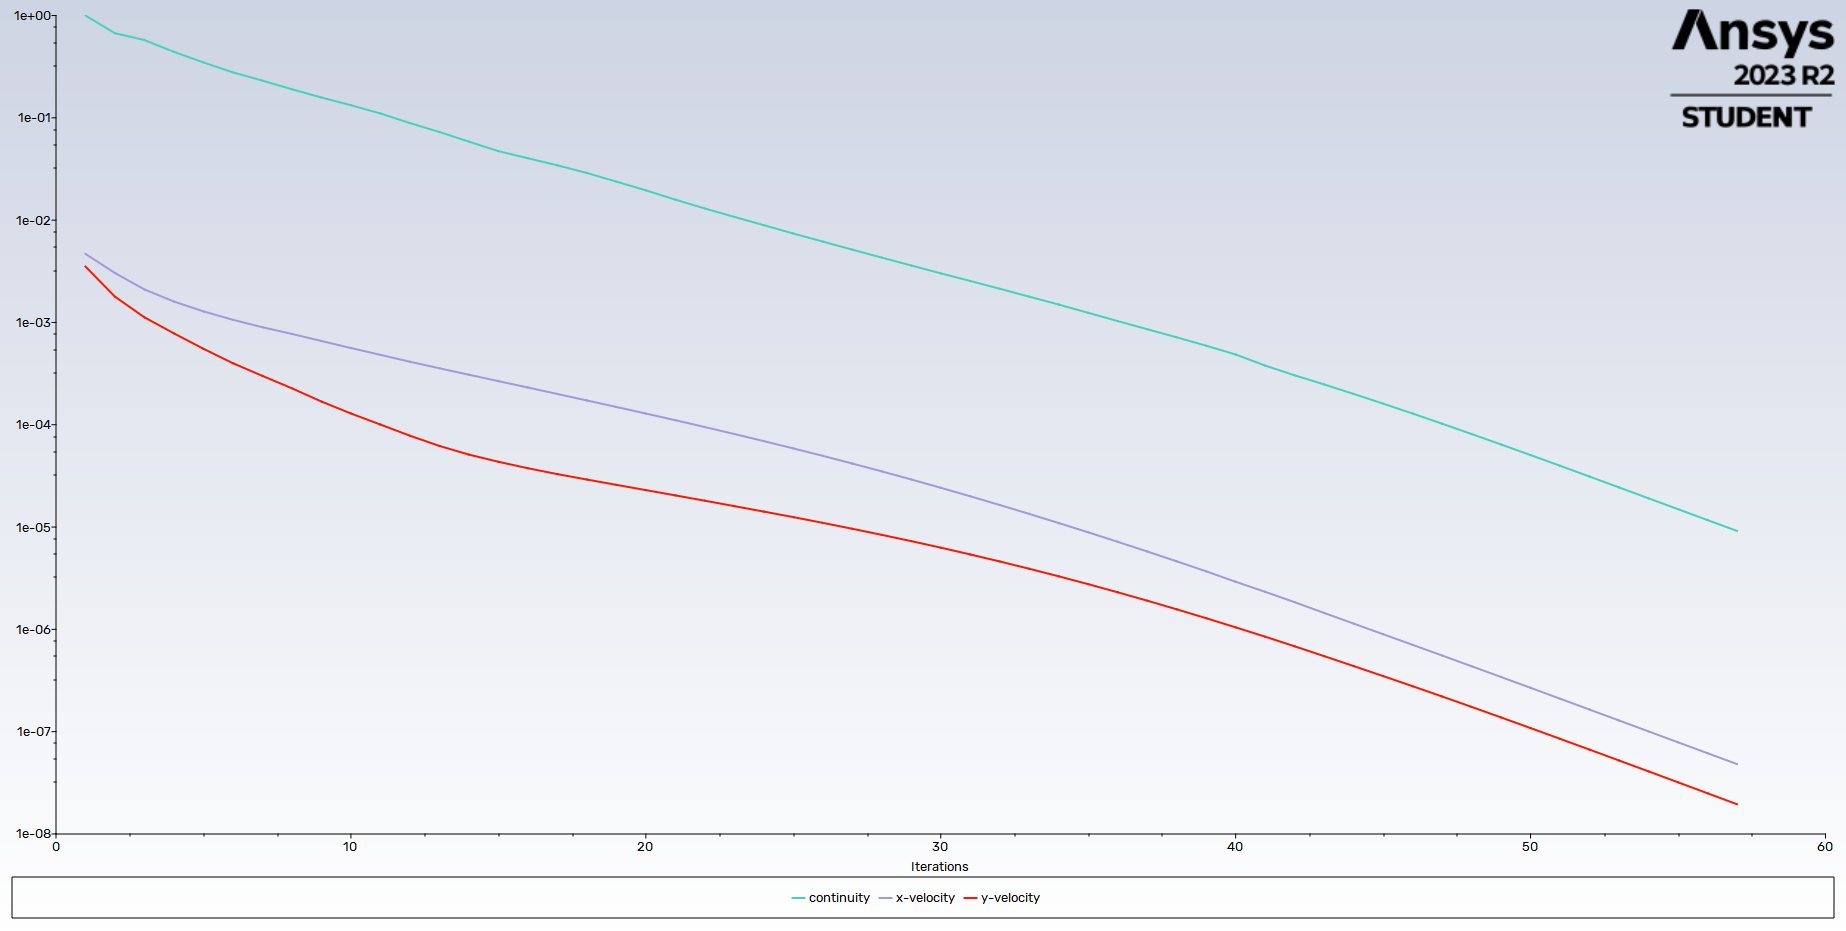
\includegraphics[width=\textwidth]{Questions/Figures/residuals grid 1.png}
        \caption{Residuals for Grid 1}
        \label{fig:residuals_grid_1}
    \end{minipage}
    \begin{minipage}{0.45\textwidth}
        \centering
        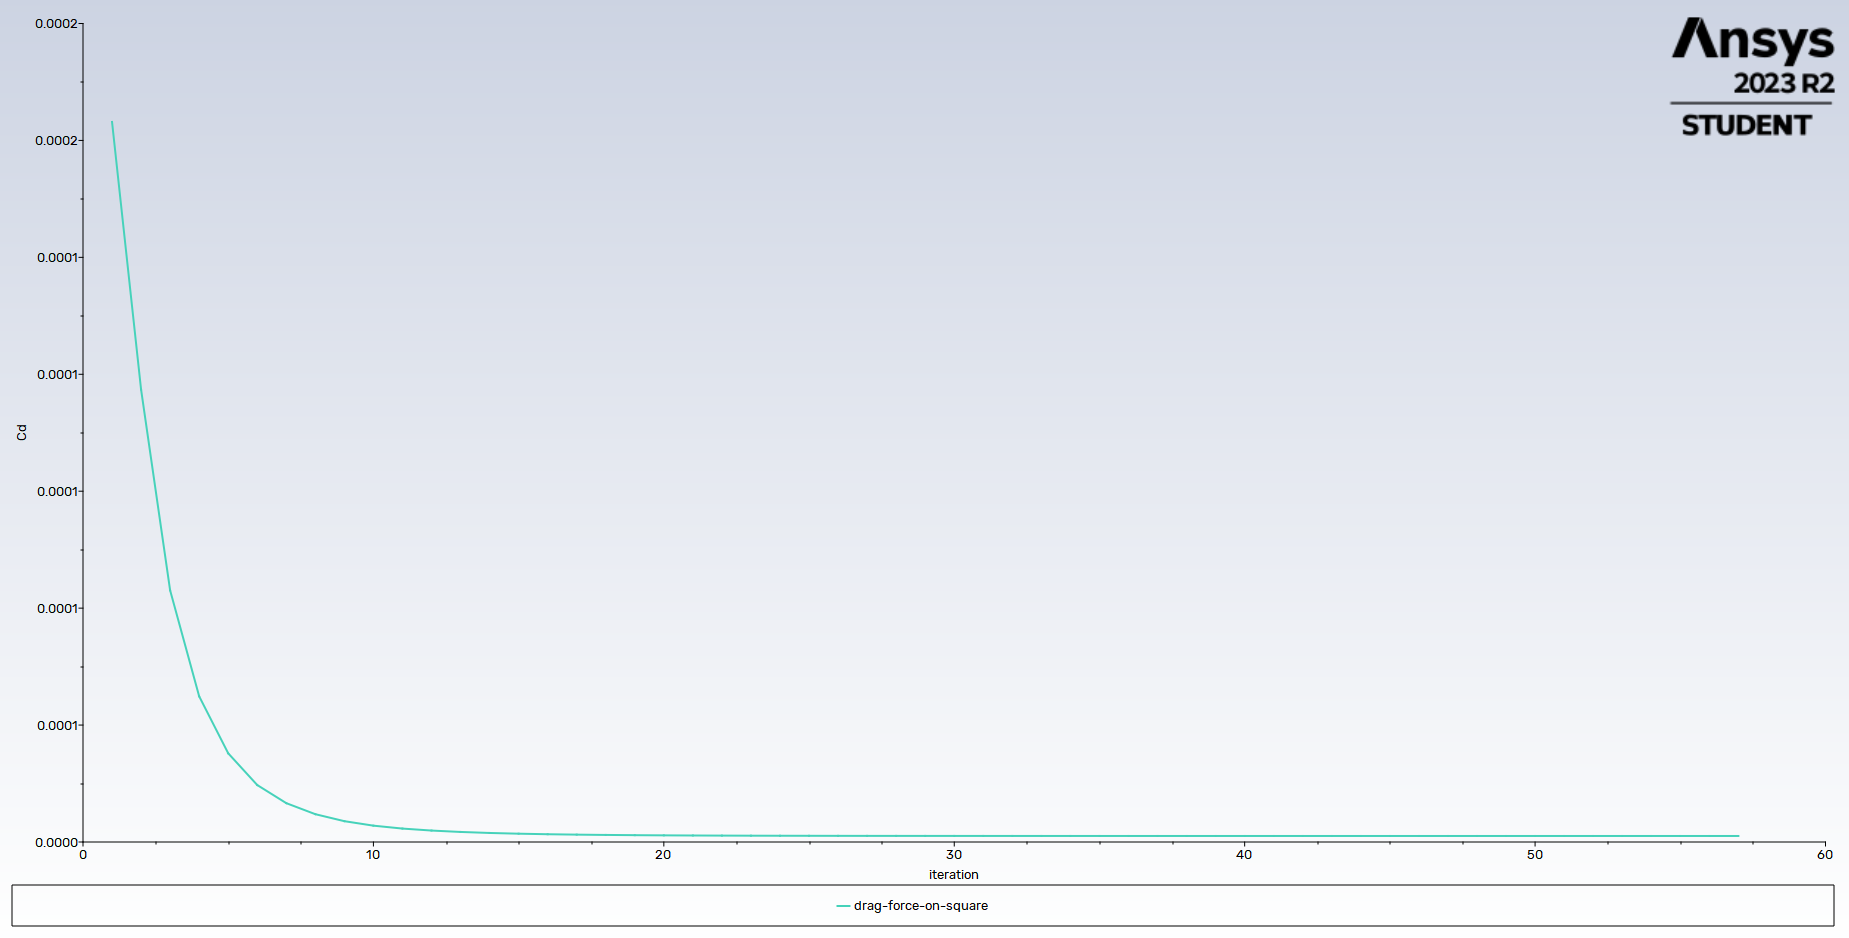
\includegraphics[width=\textwidth]{Questions/Figures/drag force on square grid 1.png}
        \caption{Drag Coefficient for Grid 1}
        \label{fig:drag_coefficient_grid_1}
    \end{minipage}
\end{figure}
\begin{figure}[H]
    \centering
    \begin{minipage}{0.45\textwidth}
        \centering
        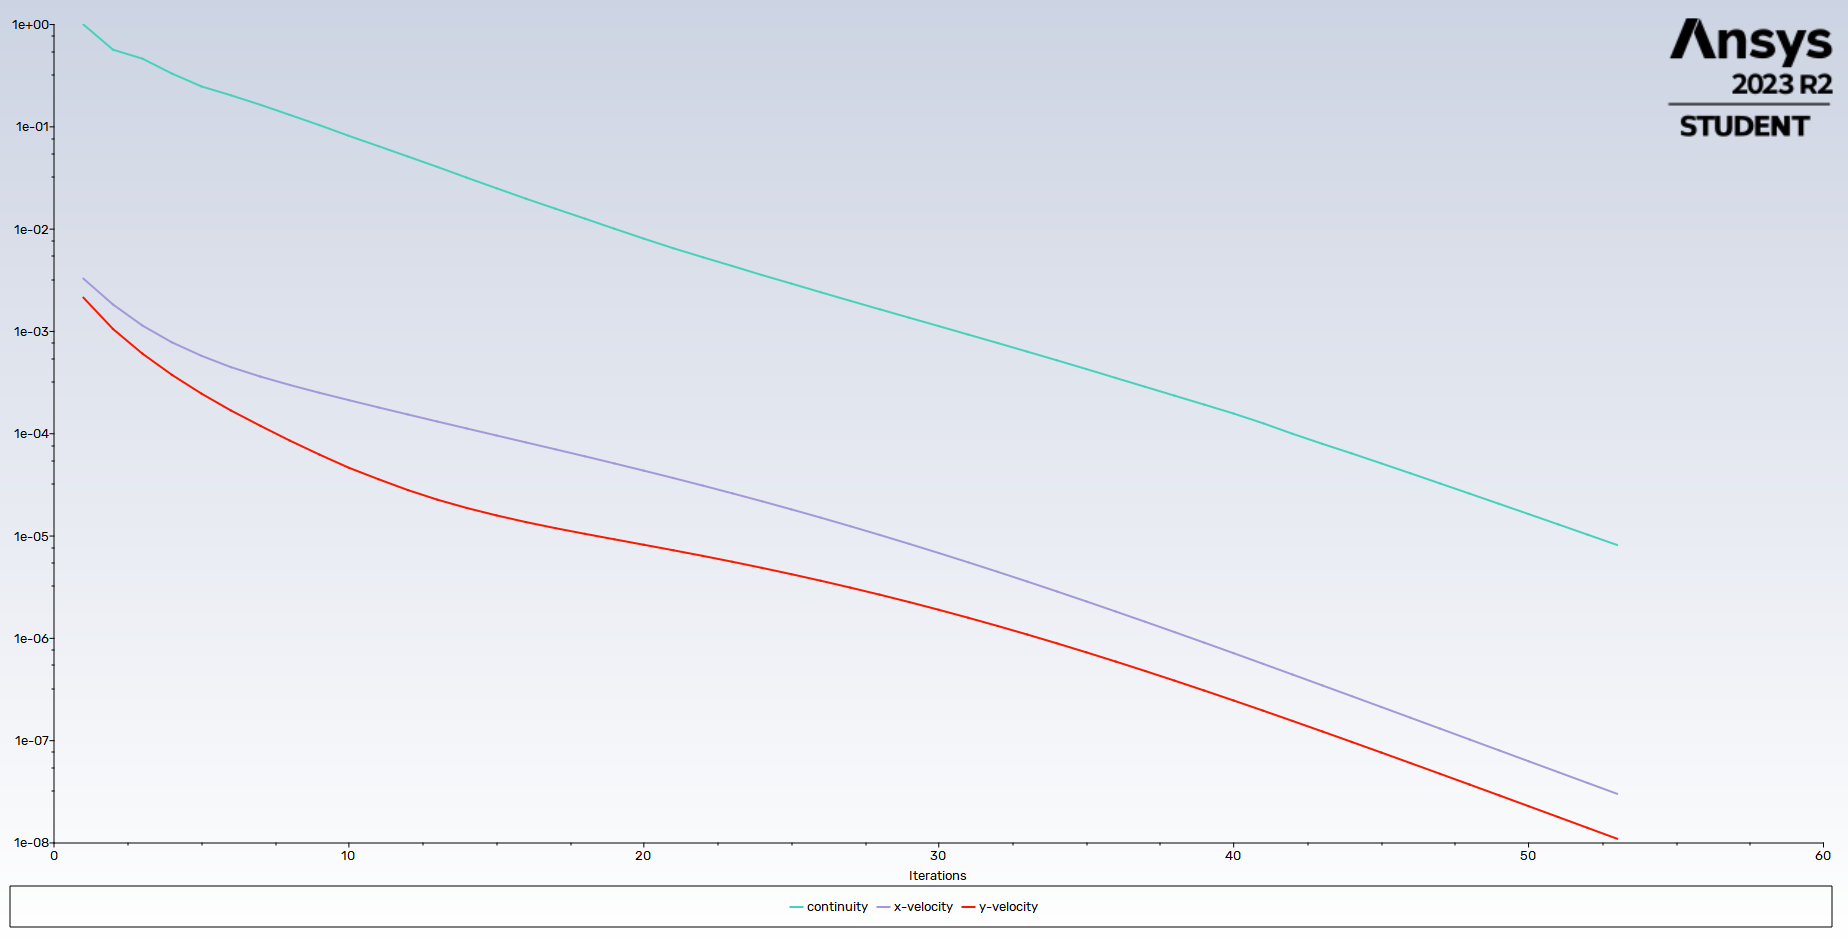
\includegraphics[width=\textwidth]{Questions/Figures/residuals grid 2.png}
        \caption{Residuals for Grid 2}
        \label{fig:residuals_grid_2}
    \end{minipage}
    \begin{minipage}{0.45\textwidth}
        \centering
        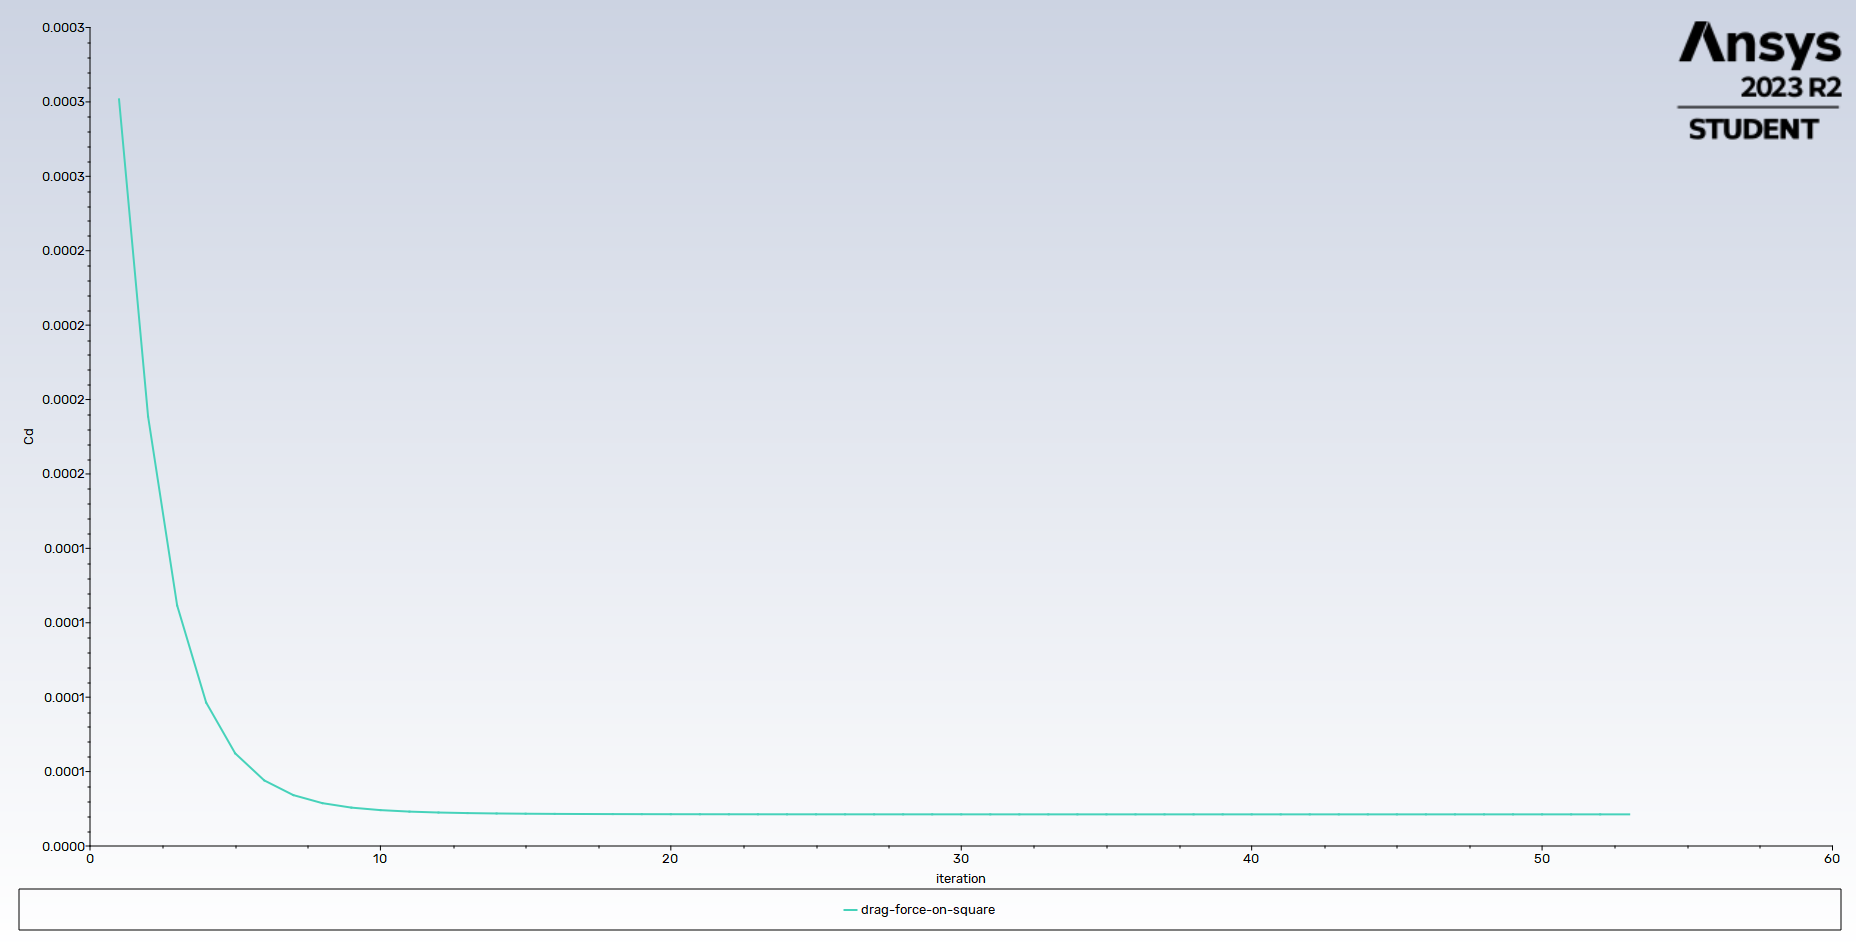
\includegraphics[width=\textwidth]{Questions/Figures/drag force on square grid 2.png}
        \caption{Drag Coefficient for Grid 2}
        \label{fig:drag_coefficient_grid_2}
    \end{minipage}
\end{figure}
\begin{figure}[H]
    \centering
    \begin{minipage}{0.45\textwidth}
        \centering
        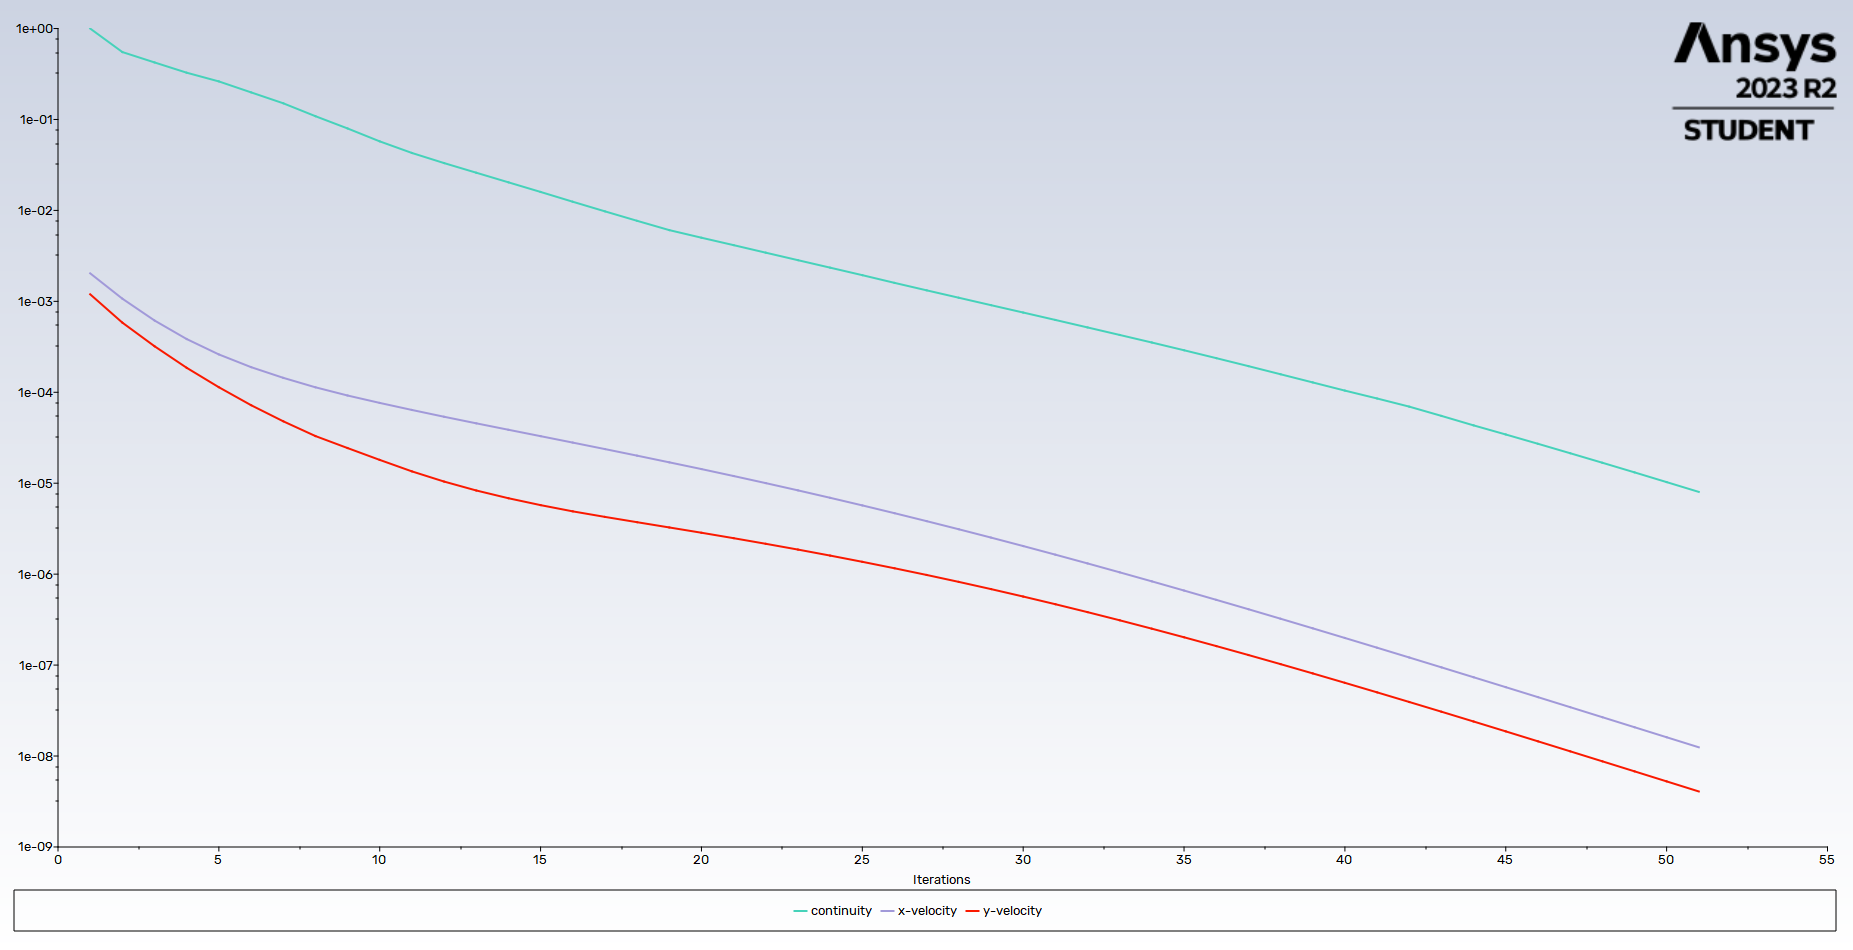
\includegraphics[width=\textwidth]{Questions/Figures/residuals grid 3.png}
        \caption{Residuals for Grid 3}
        \label{fig:residuals_grid_3}
    \end{minipage}
    \begin{minipage}{0.45\textwidth}
        \centering
        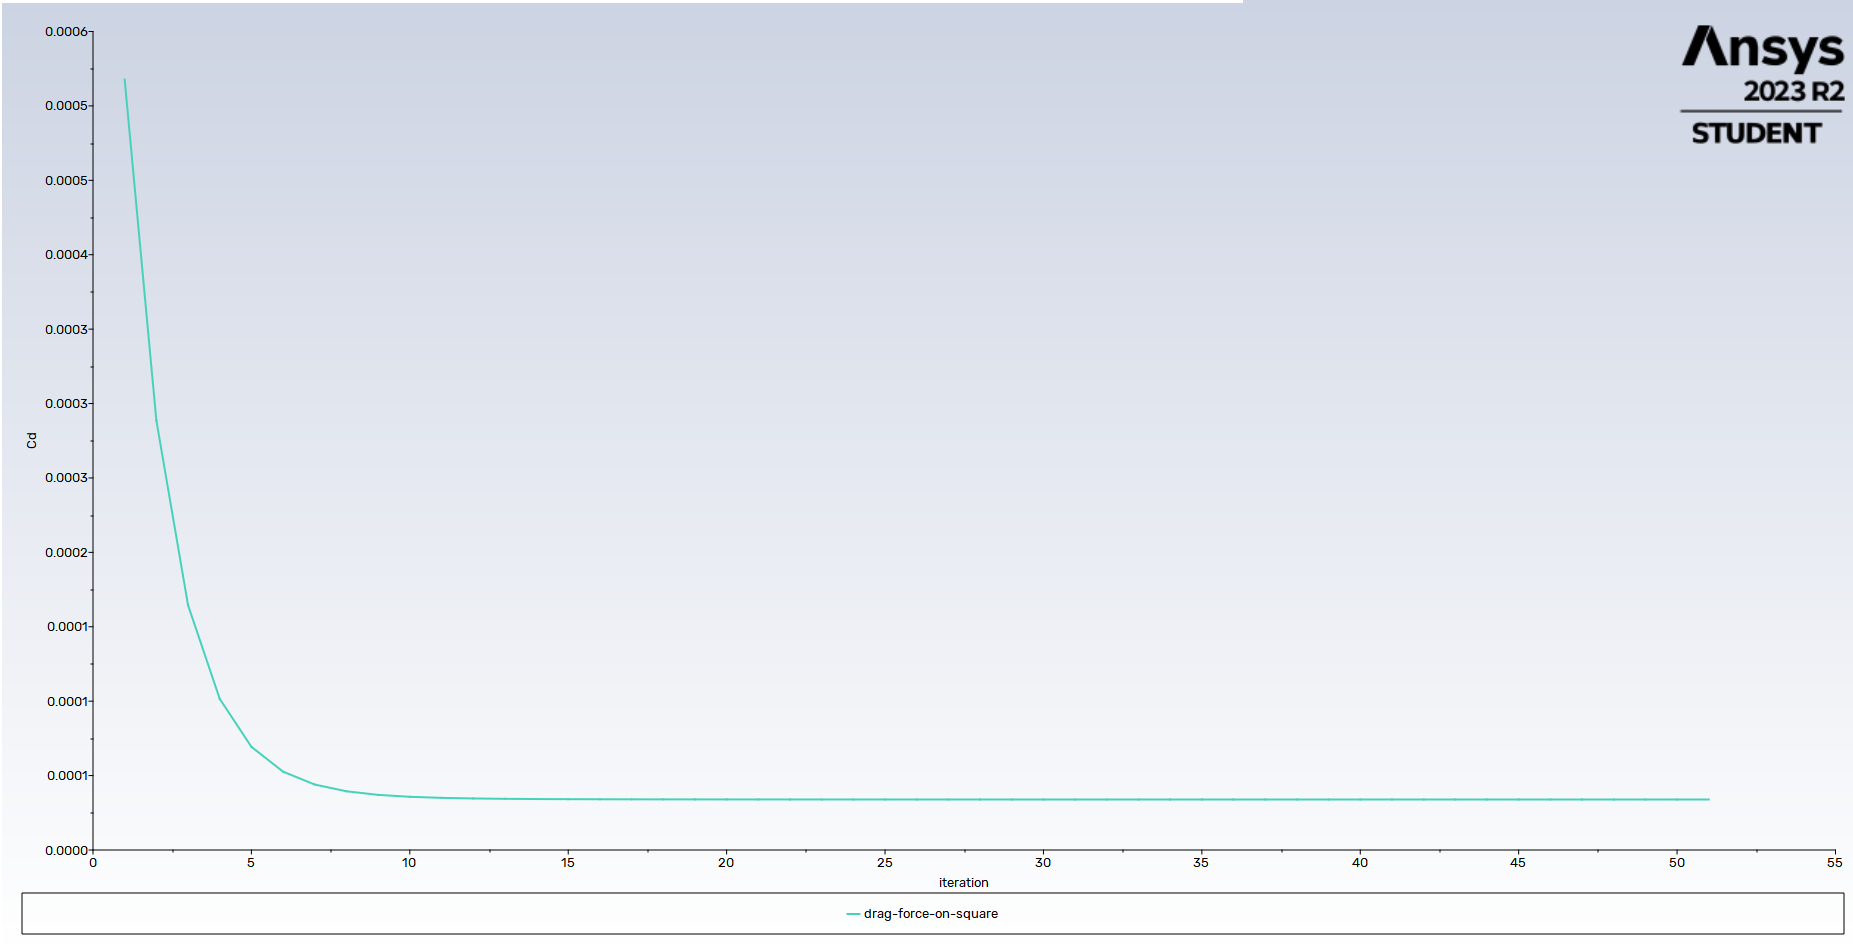
\includegraphics[width=\textwidth]{Questions/Figures/drag force on square grid 3.png}
        \caption{Drag Coefficient for Grid 3}
        \label{fig:drag_coefficient_grid_3}
    \end{minipage}
\end{figure}
\begin{figure}[H]
    \centering
    \begin{minipage}{0.45\textwidth}
        \centering
        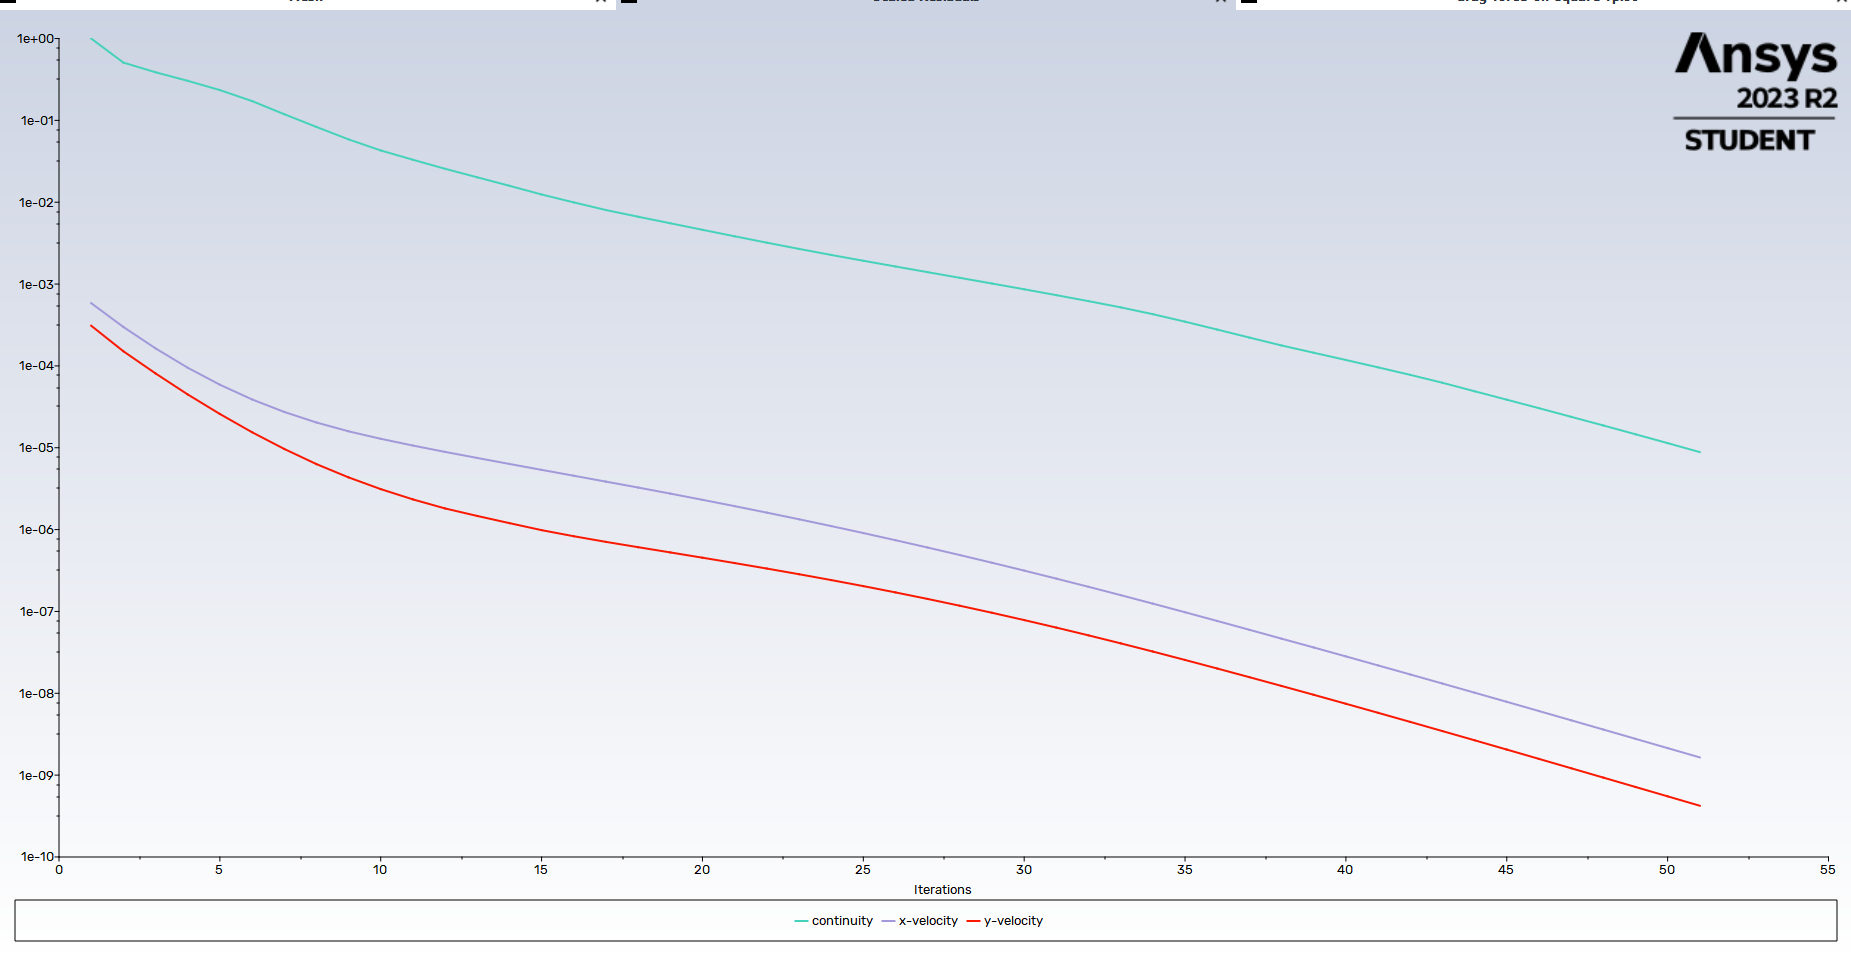
\includegraphics[width=\textwidth]{Questions/Figures/residuals grid 4.png}
        \caption{Residuals for Grid 4}
        \label{fig:residuals_grid_4}
    \end{minipage}
    \begin{minipage}{0.45\textwidth}
        \centering
        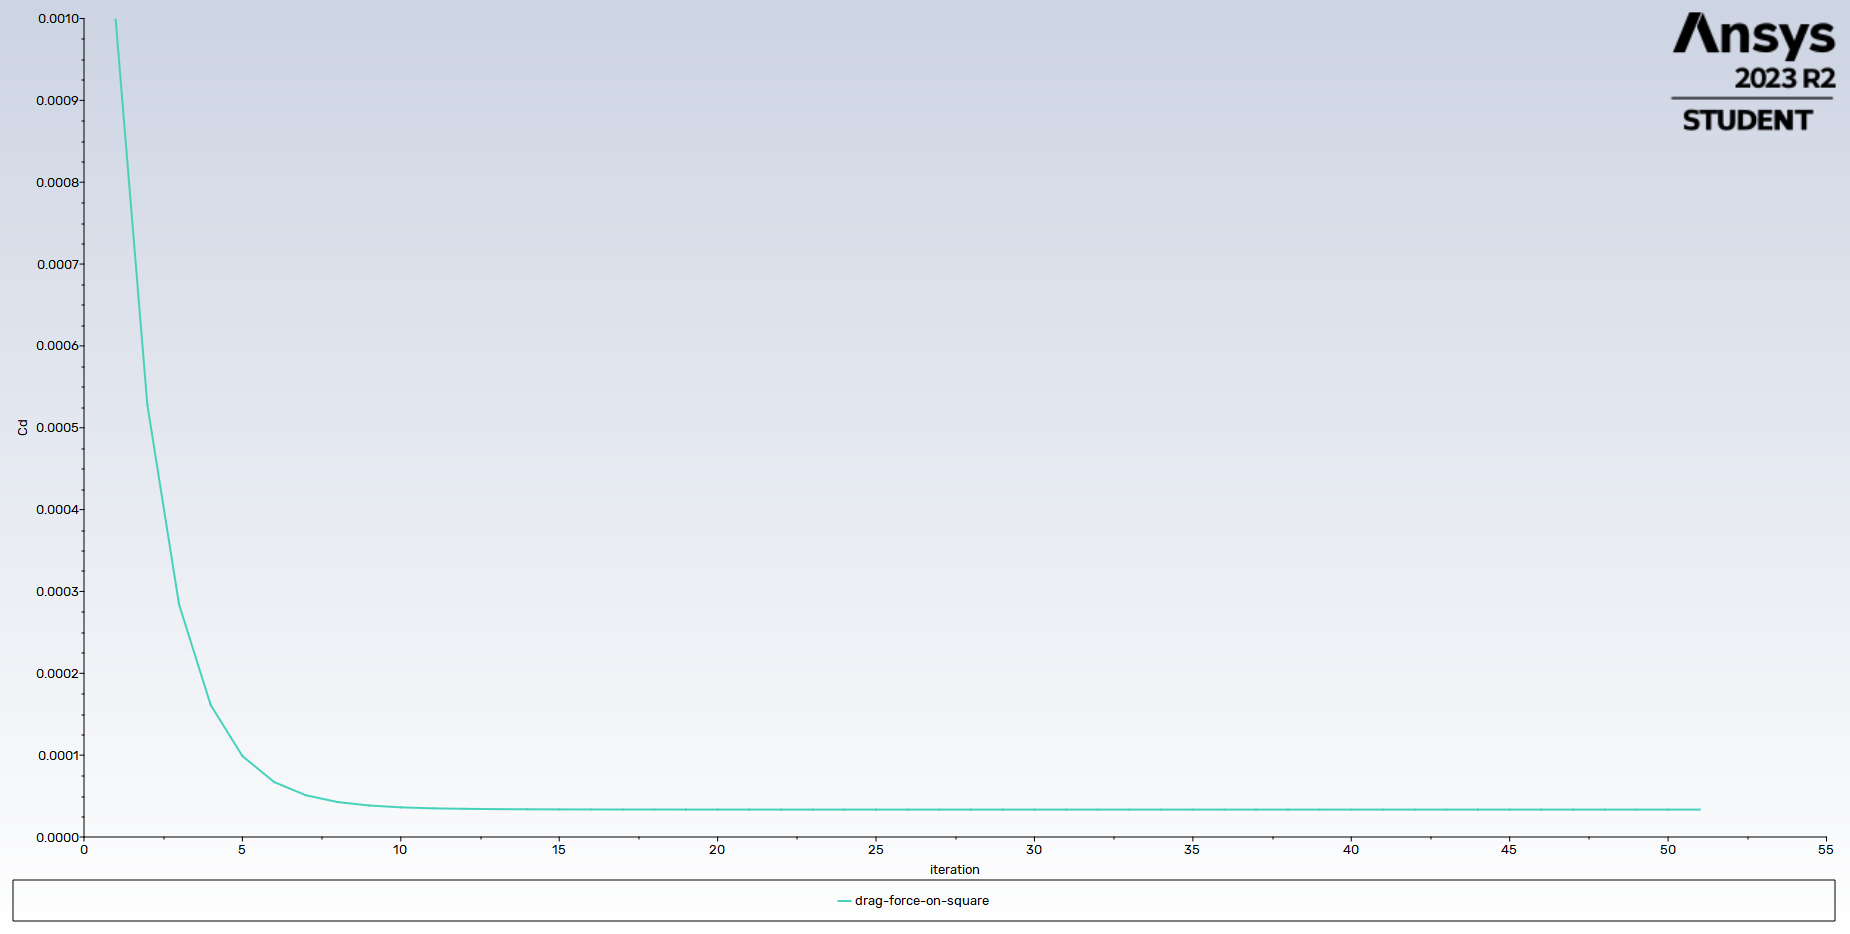
\includegraphics[width=\textwidth]{Questions/Figures/drag force on square grid 4.png}
        \caption{Drag Coefficient for Grid 4}
        \label{fig:drag_coefficient_grid_4}
    \end{minipage}
\end{figure}
\begin{figure}[H]
    \centering
    \begin{minipage}{0.45\textwidth}
        \centering
        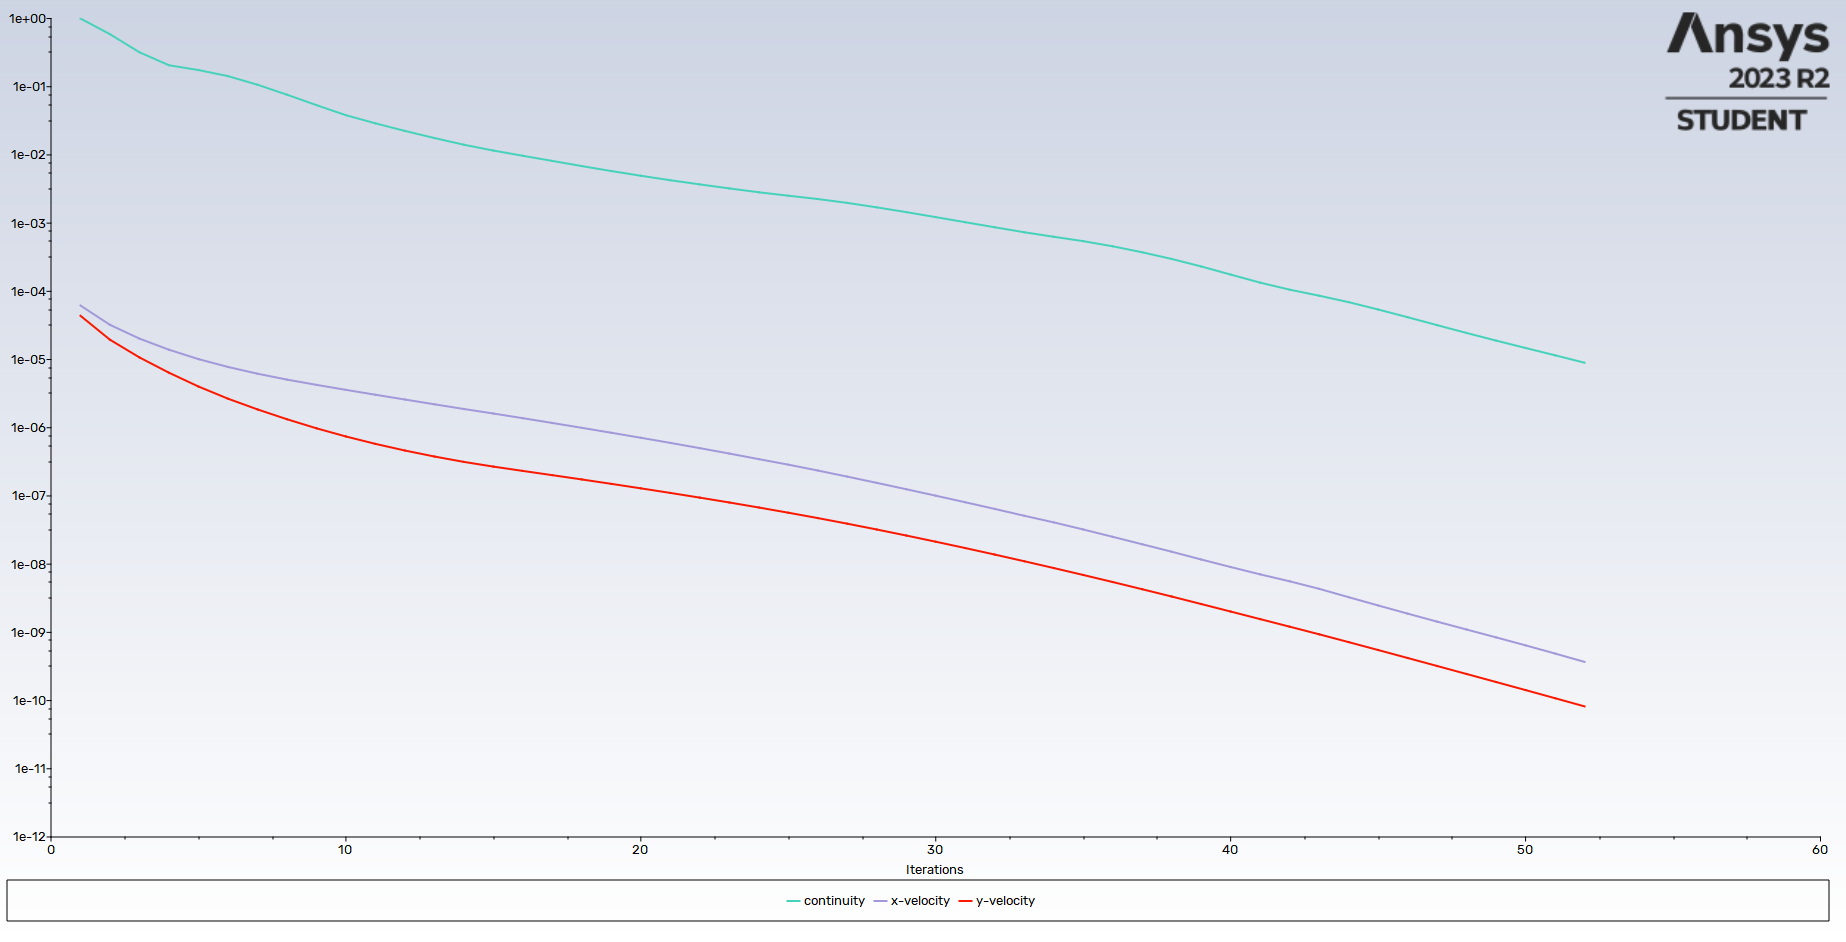
\includegraphics[width=\textwidth]{Questions/Figures/residuals grid 5.png}
        \caption{Residuals for Grid 5}
        \label{fig:residuals_grid_5}
    \end{minipage}
    \begin{minipage}{0.45\textwidth}
        \centering
        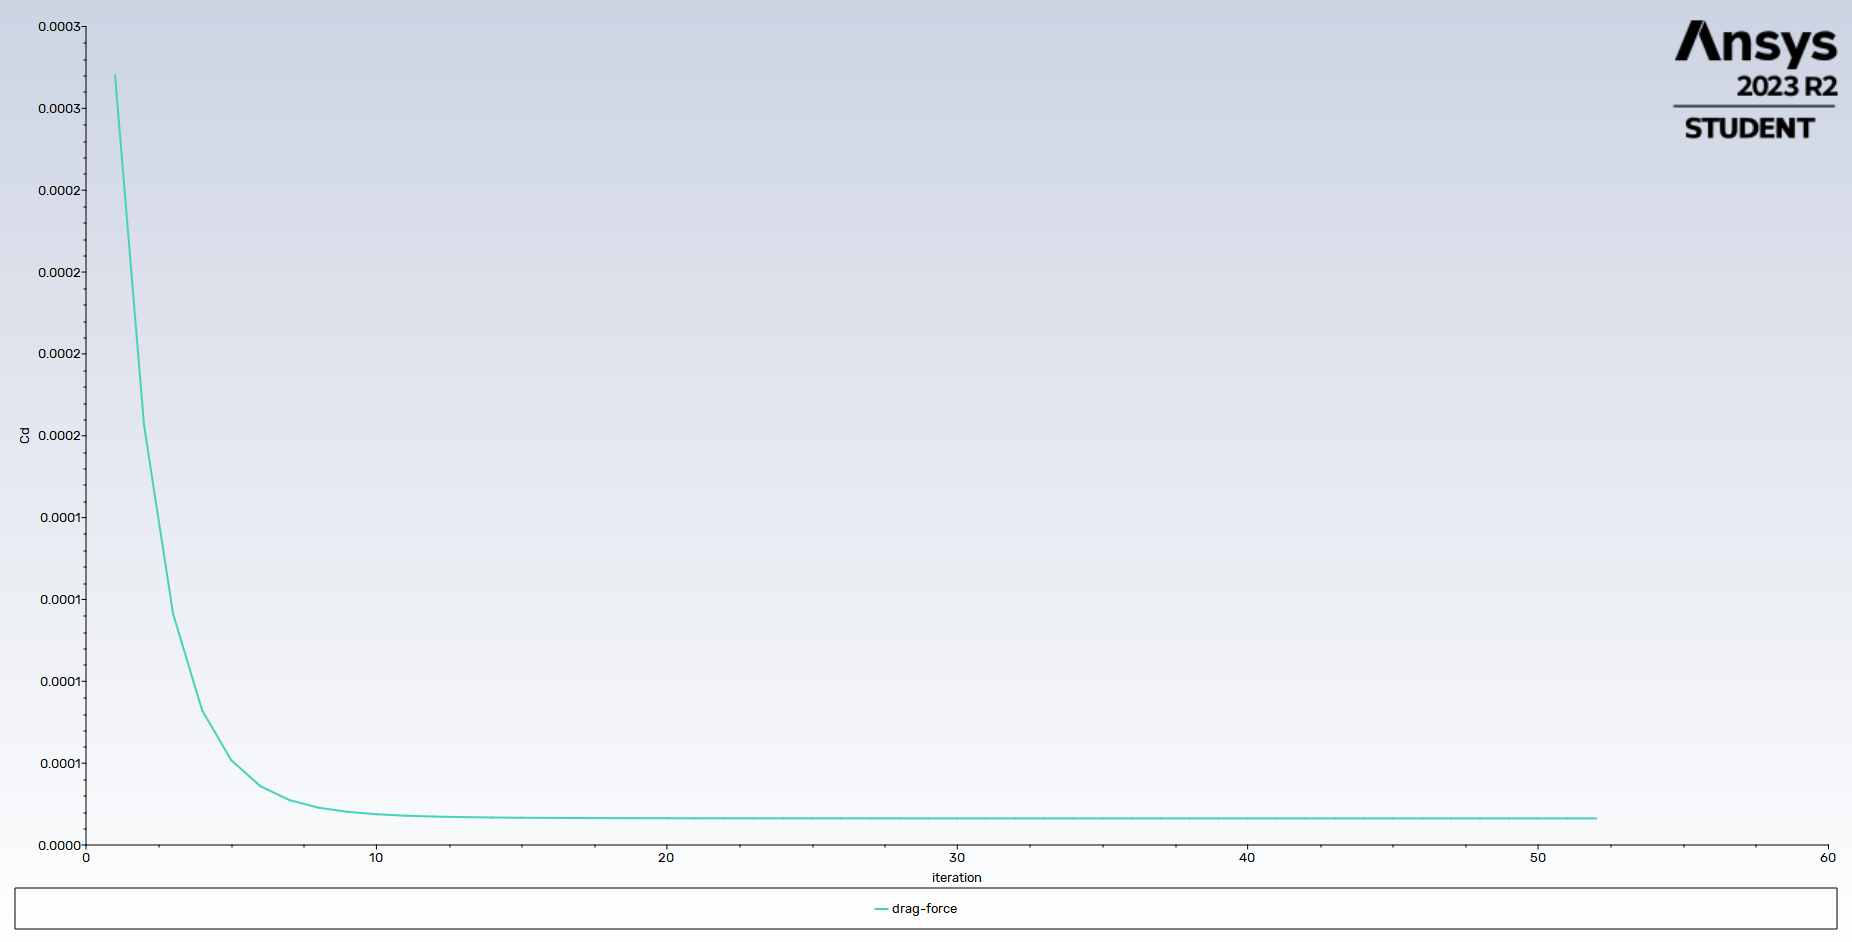
\includegraphics[width=\textwidth]{Questions/Figures/drag force on square grid 5.png}
        \caption{Drag Coefficient for Grid 5}
        \label{fig:drag_coefficient_grid_5}
    \end{minipage}
\end{figure}
\begin{figure}[H]
    \centering
    \begin{minipage}{0.45\textwidth}
        \centering
        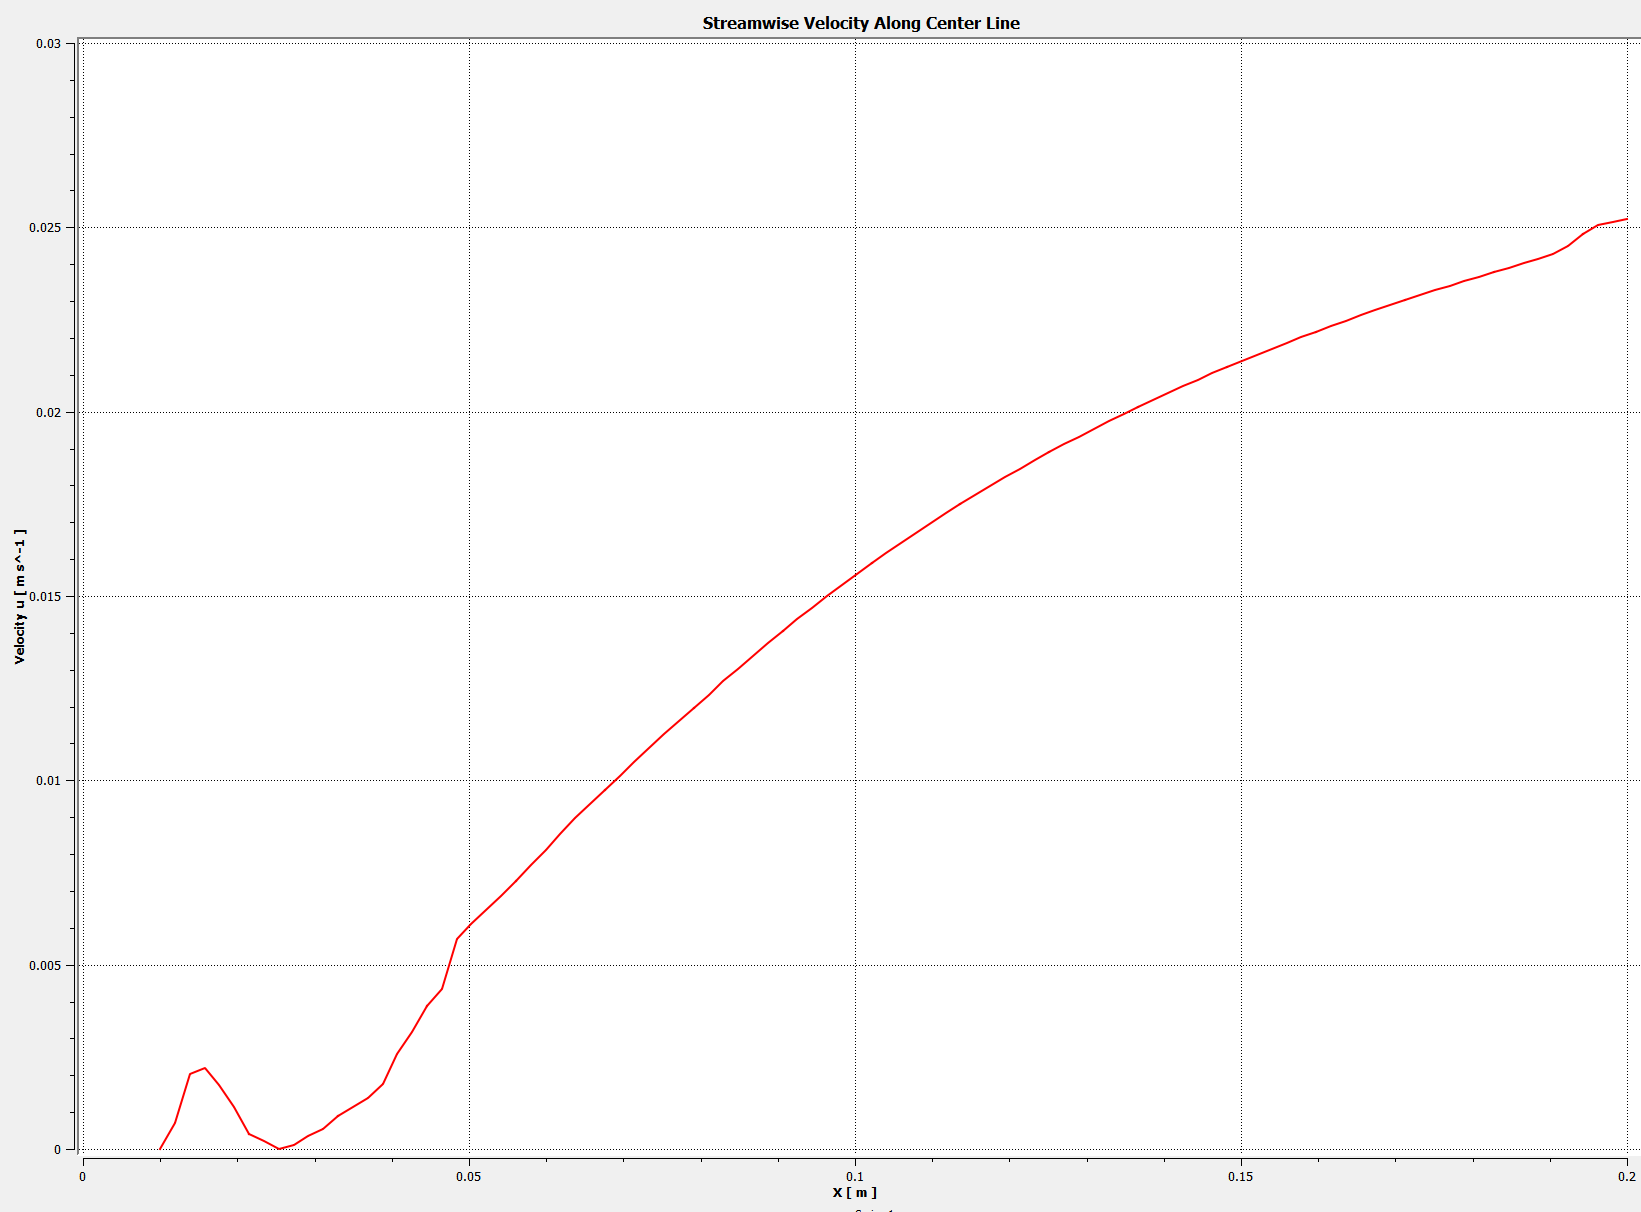
\includegraphics[width=\textwidth]{Questions/Figures/u velocity along centerline grid 1.png}
        \caption{Velocity Profile for Grid 1}
        \label{fig:velocity_profile_grid_1}
    \end{minipage}
    \begin{minipage}{0.45\textwidth}
        \centering
        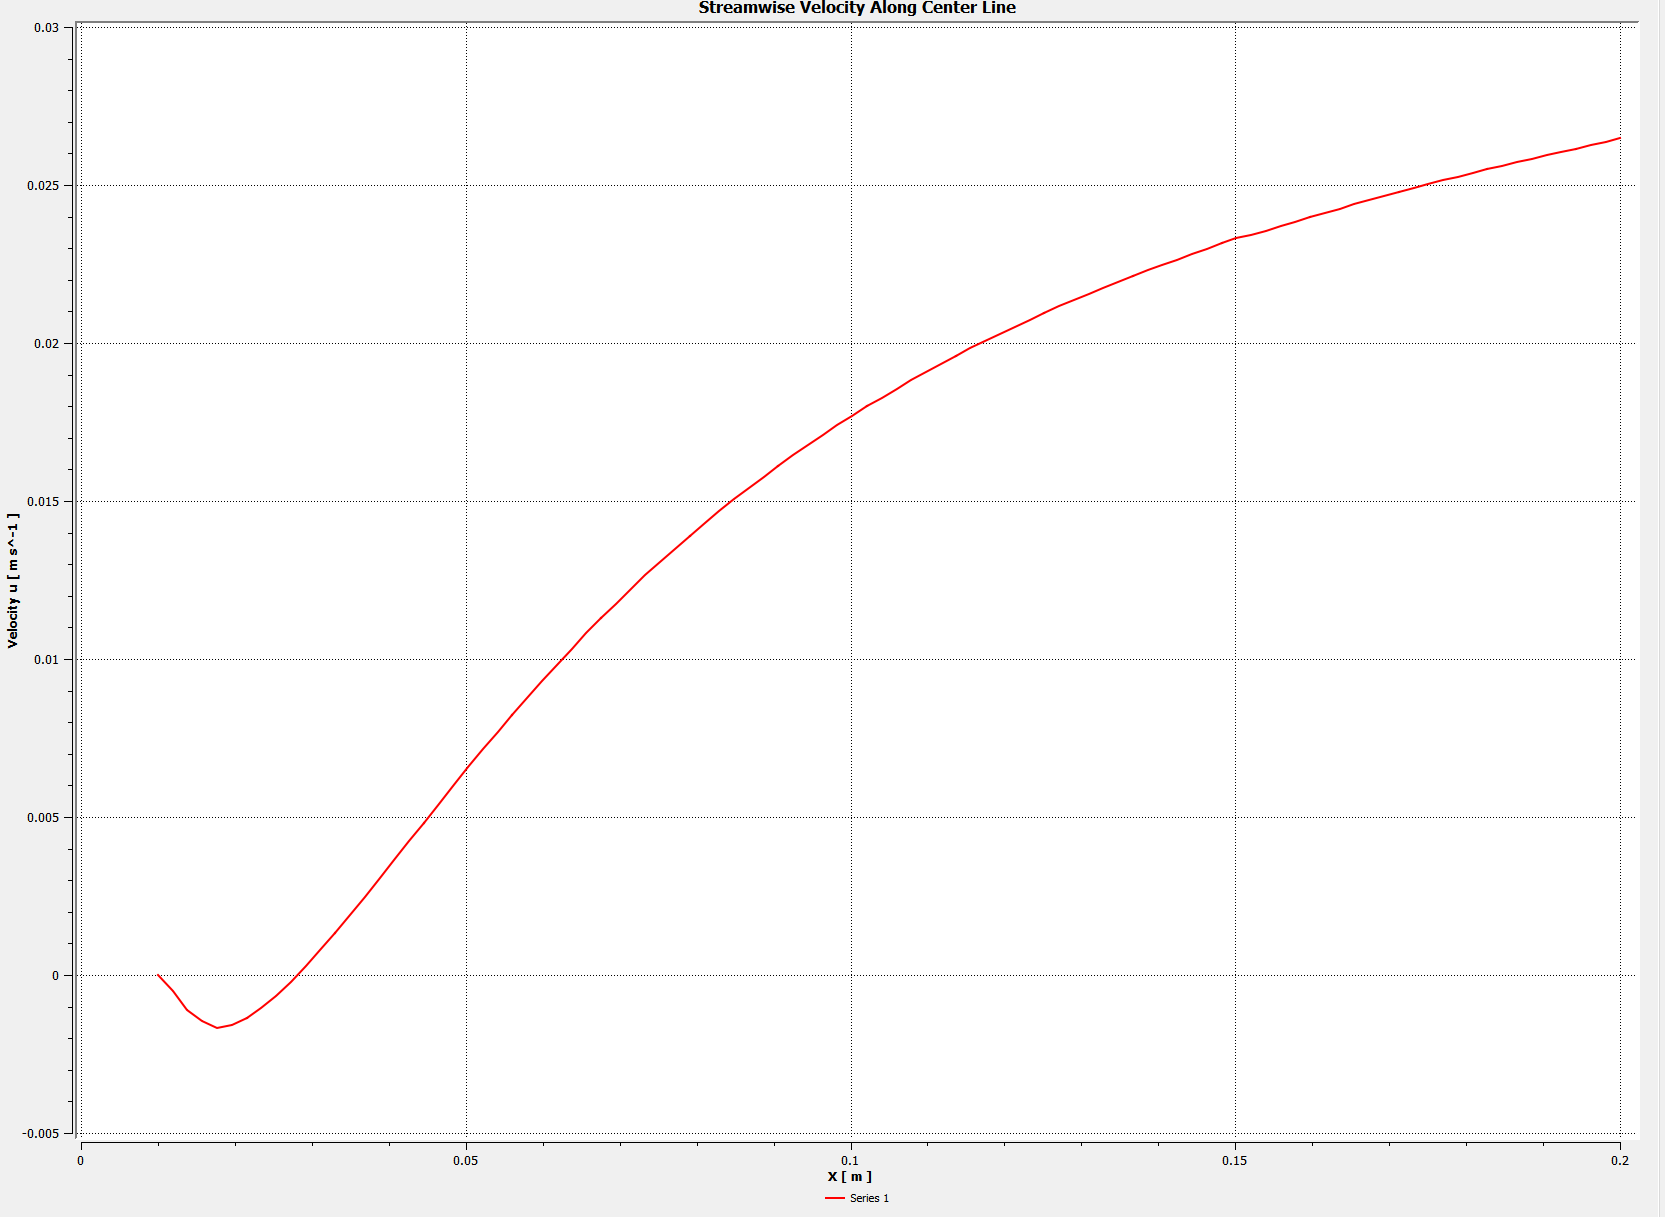
\includegraphics[width=\textwidth]{Questions/Figures/u velocity along centerline grid 2.png}
        \caption{Velocity Profile for Grid 2}
        \label{fig:velocity_profile_grid_2}
    \end{minipage}
\end{figure}
\begin{figure}[H]
    \centering
    \begin{minipage}{0.45\textwidth}
        \centering
        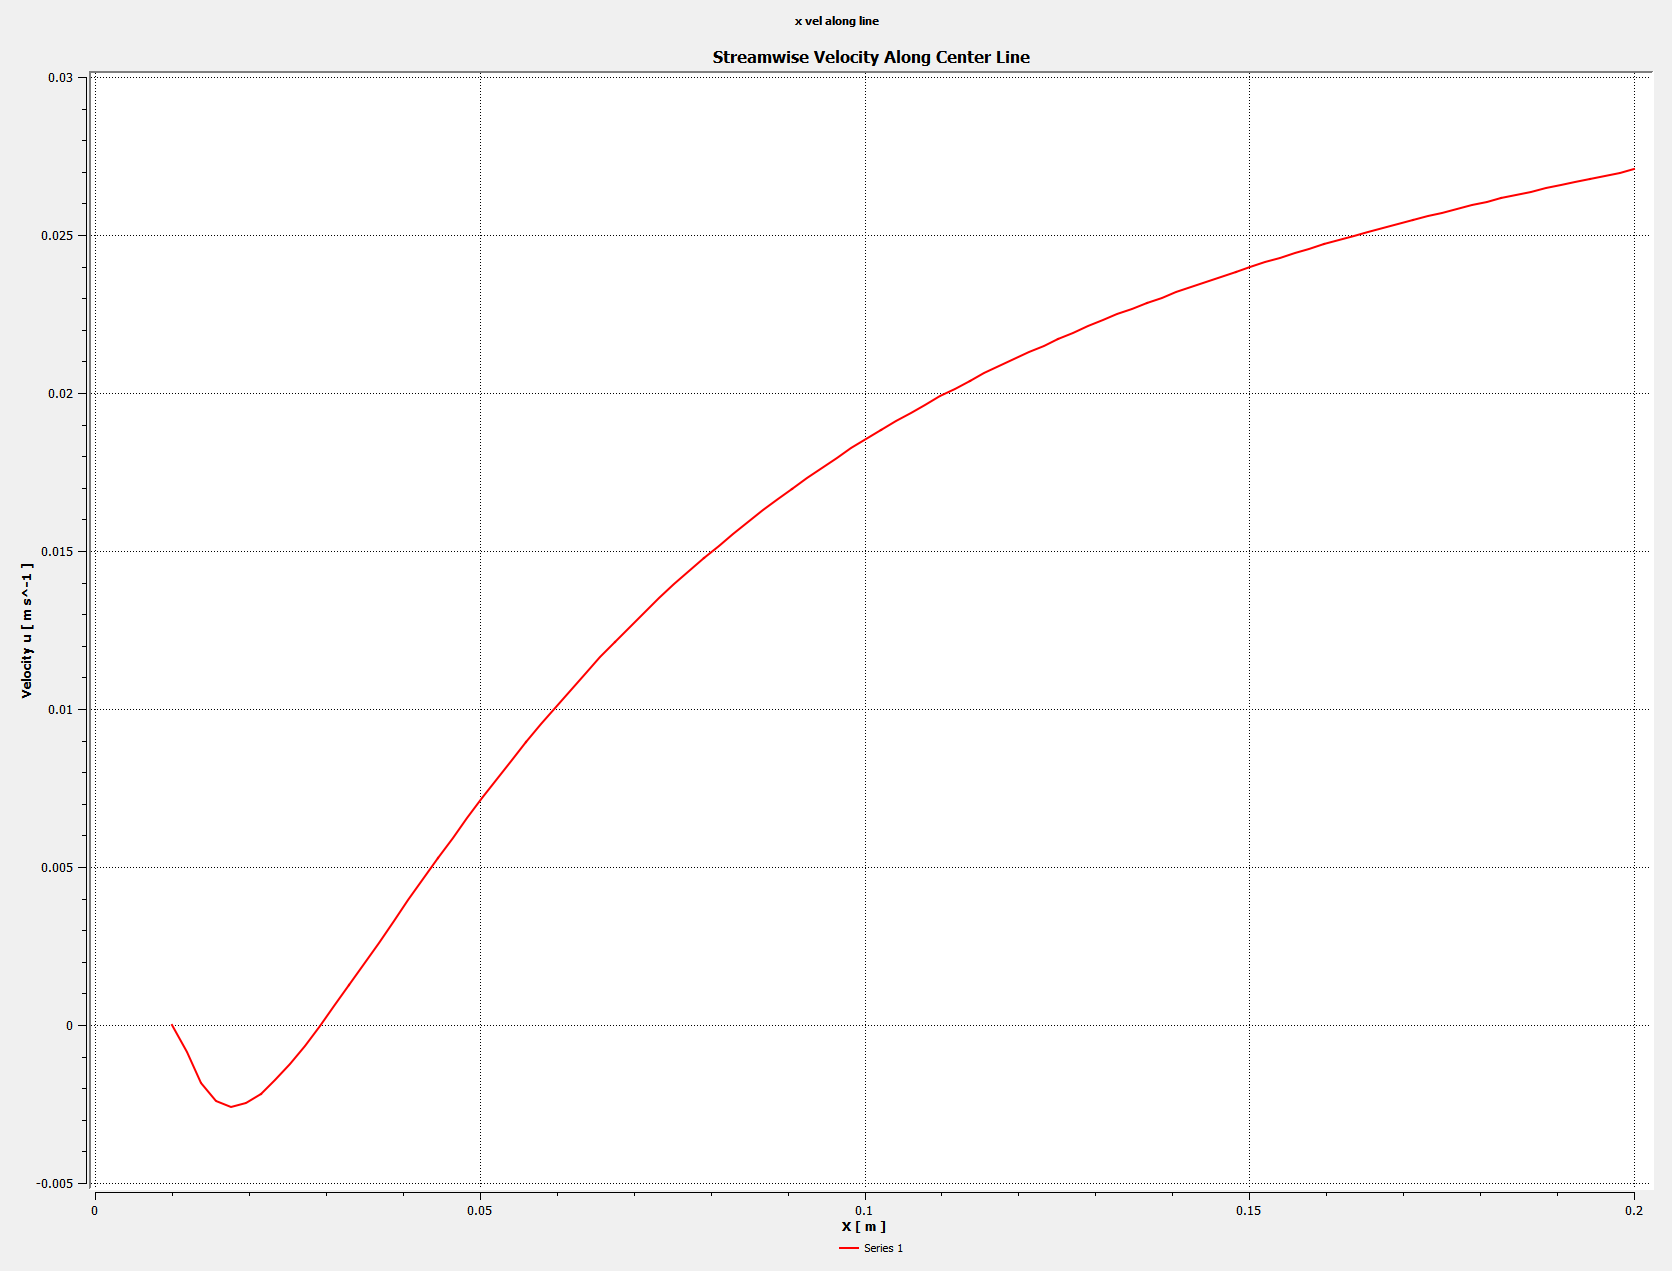
\includegraphics[width=\textwidth]{Questions/Figures/u velocity along centerline grid 3.png}
        \caption{Velocity Profile for Grid 3}
        \label{fig:velocity_profile_grid_3}
    \end{minipage}
    \begin{minipage}{0.45\textwidth}
        \centering
        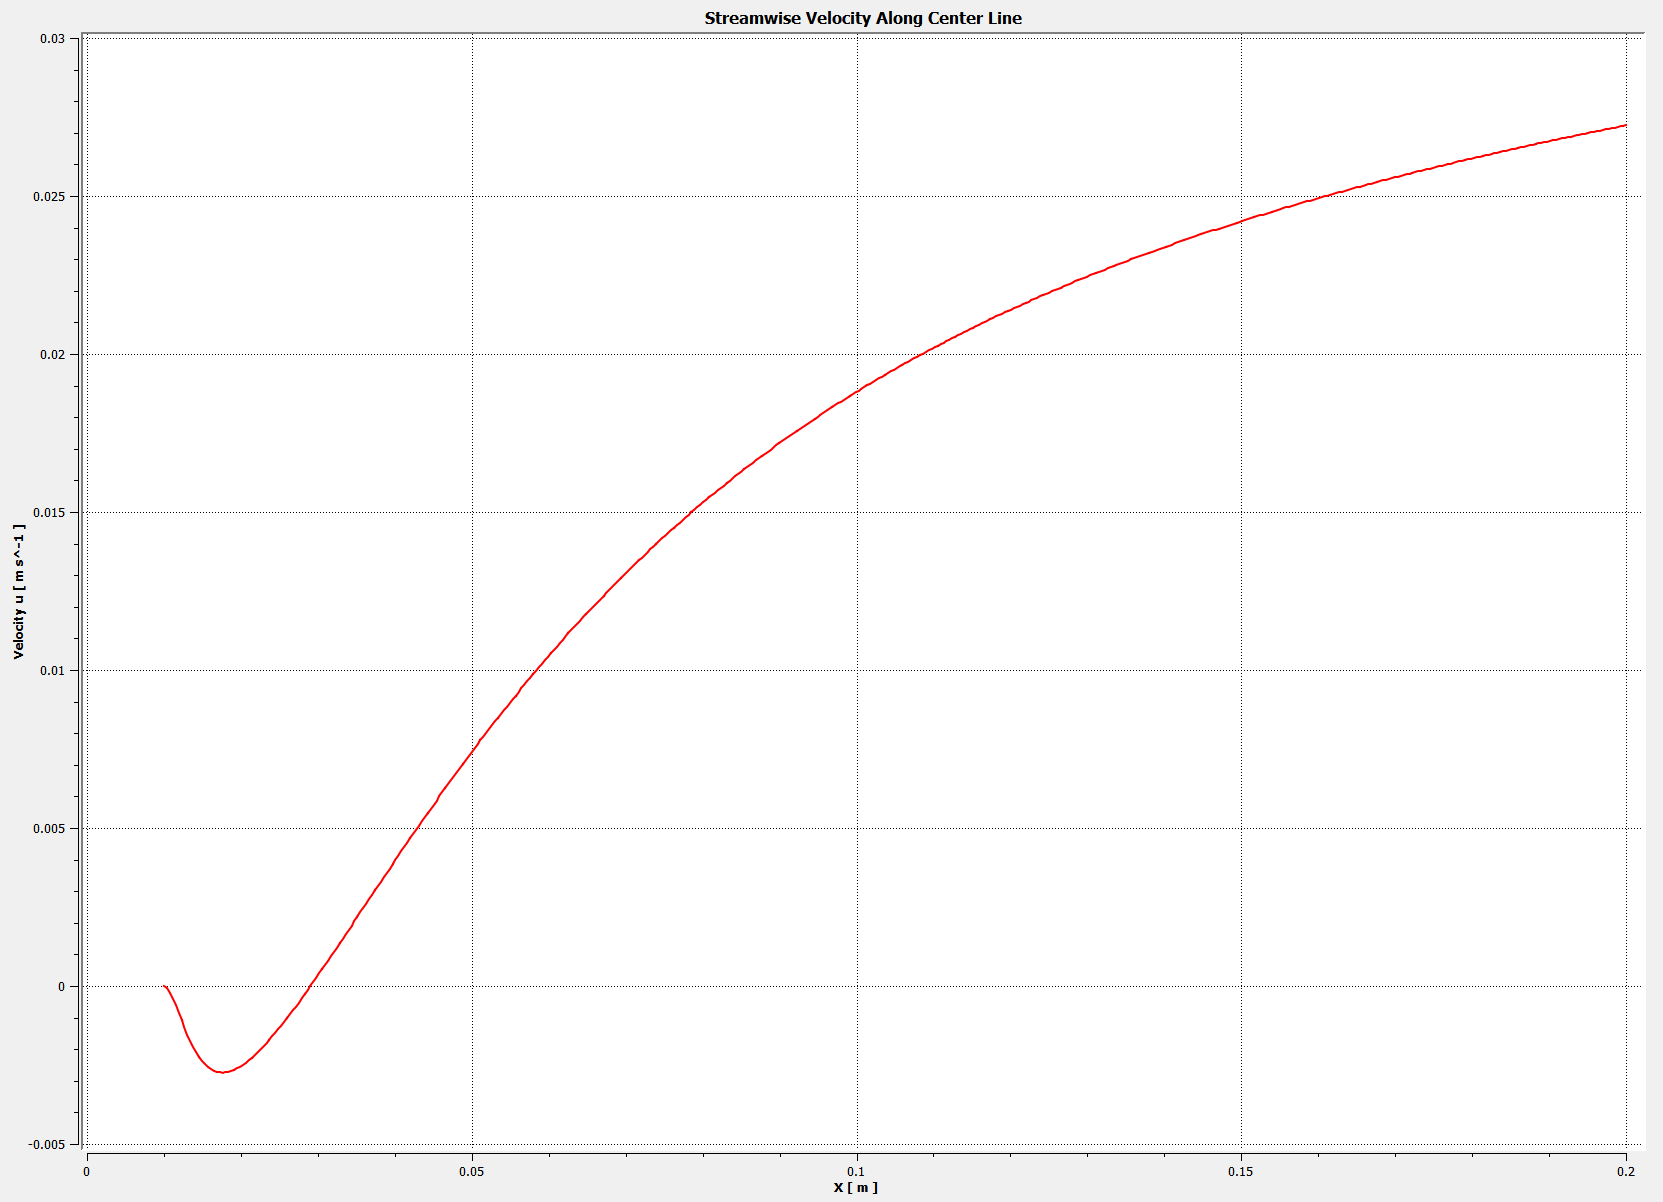
\includegraphics[width=\textwidth]{Questions/Figures/u velocity along centerline grid 4.png}
        \caption{Velocity Profile for Grid 4}
        \label{fig:velocity_profile_grid_4}
    \end{minipage}
\end{figure}
\begin{figure}[H]
    \centering
    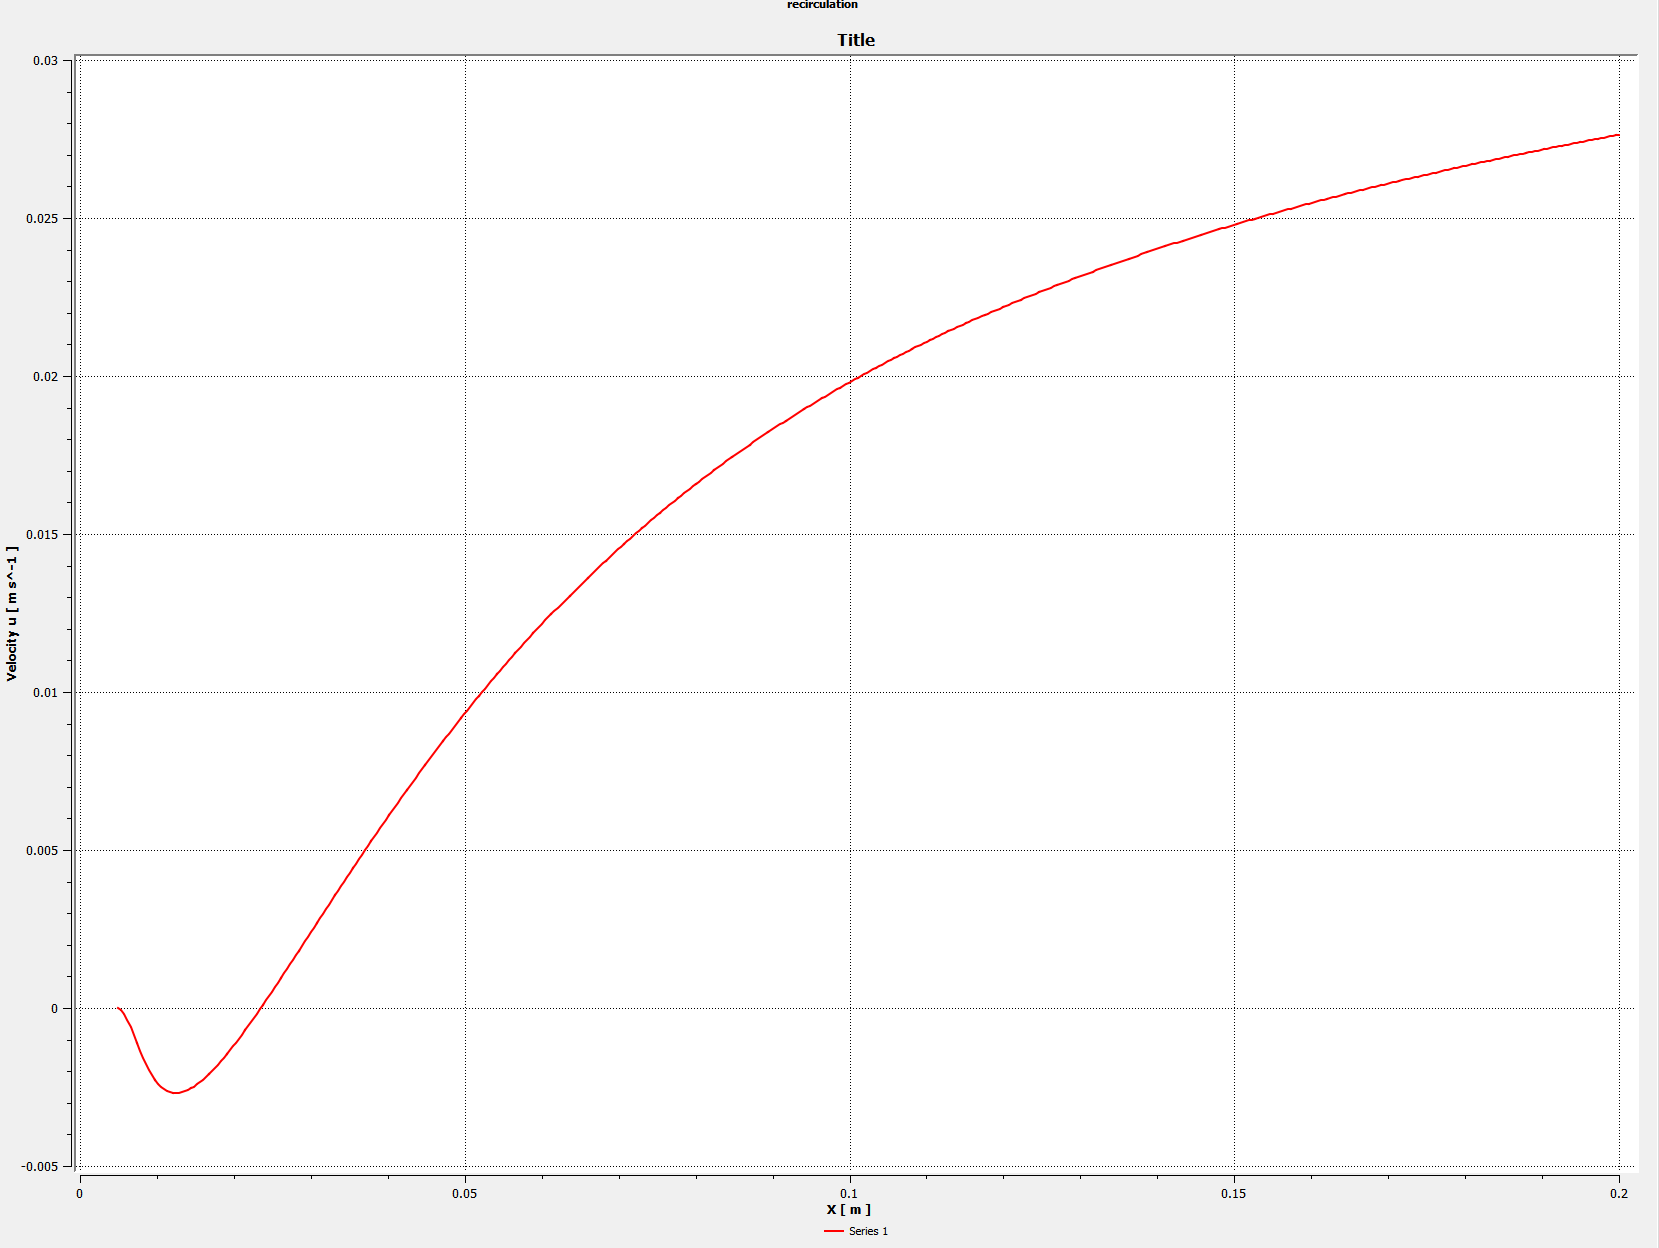
\includegraphics[width=0.45\textwidth]{Questions/Figures/u velocity along centerline grid 5.png}
    \caption{Velocity Profile for Grid 5}
    \label{fig:velocity_profile_grid_5}
\end{figure}

\subsection{Analyses of the Velocity Fields}
The contours are shown in Figures \ref{fig:velocity_contour_grid_1} and \ref{fig:velocity_contour_grid_5}. The flow is symmetric about the centerline. The flow behind the square object is observable in grid 1, but much more refined in grid 5. In grid 5, two flanges of high velocity flow can be seen to the side of the square object. In comparison, the whole region to the side of the square object is a high velocity region in grid 1, which makes less physical sense. Grid 5 should be used since the results are more physical.

The streamlines are shown in Figures \ref{fig:streamlines_grid_1}, \ref{fig:streamlines_grid_3}, and \ref{fig:streamlines_grid_5}. Again, the flow is symmetric about the centerline. A small vortex region can be seen from behind the square object in grids 3 and 5. The flow aspects are difficult to discern in grid 1. Considering that meshing grid 5 took roughly 20 minutes to mesh on my desktop computer, grid 3 is a good compromise between accuracy and computational cost.

\begin{figure}[H]
    \centering
    \begin{minipage}{0.45\textwidth}
        \centering
        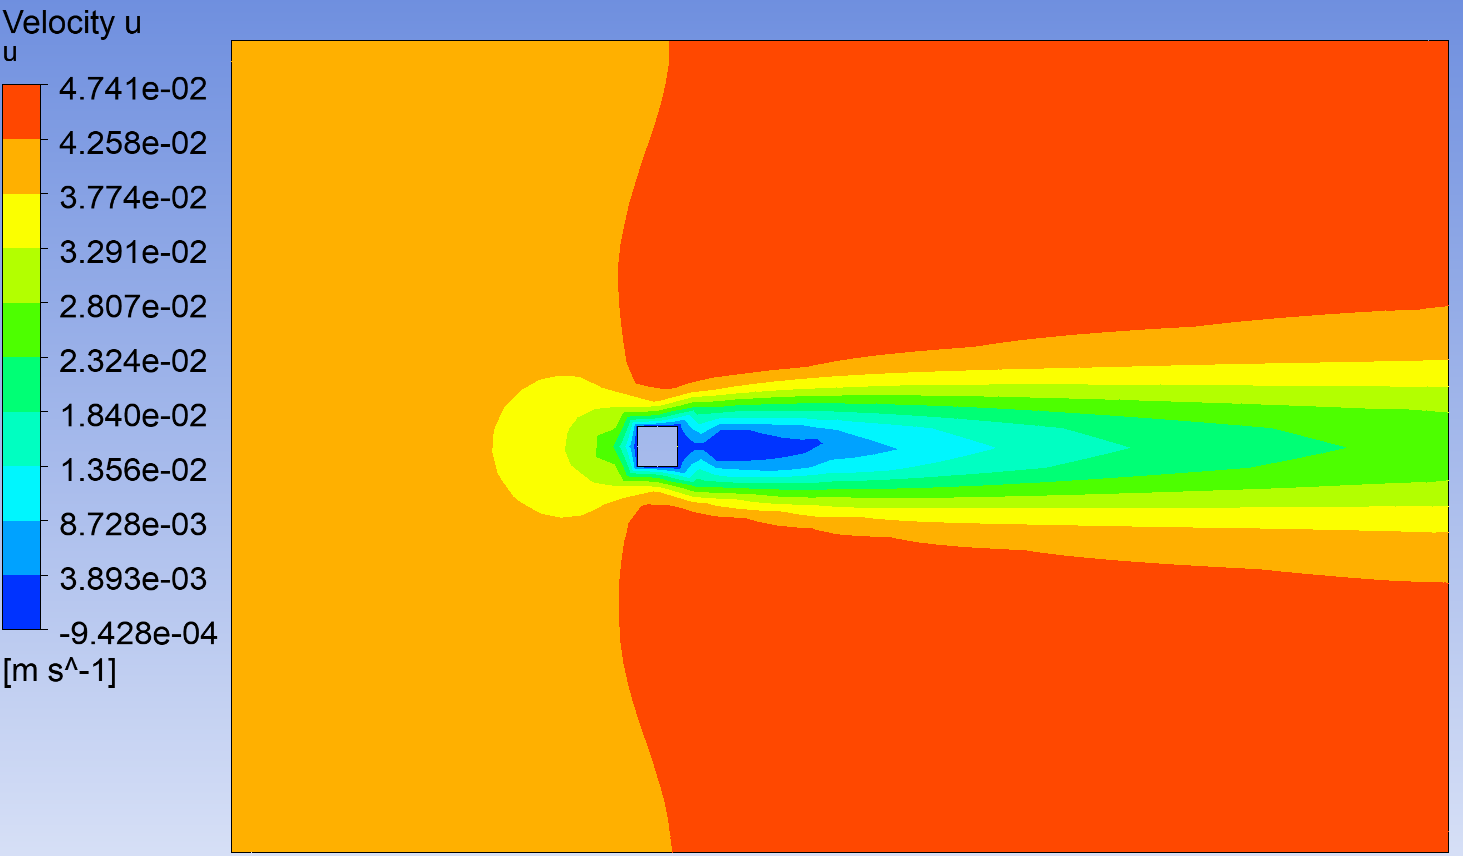
\includegraphics[width=\textwidth]{Questions/Figures/u velocity contour grid 1.png}
        \caption{Velocity Contour for Grid 1}
        \label{fig:velocity_contour_grid_1}
    \end{minipage}
    \begin{minipage}{0.45\textwidth}
        \centering
        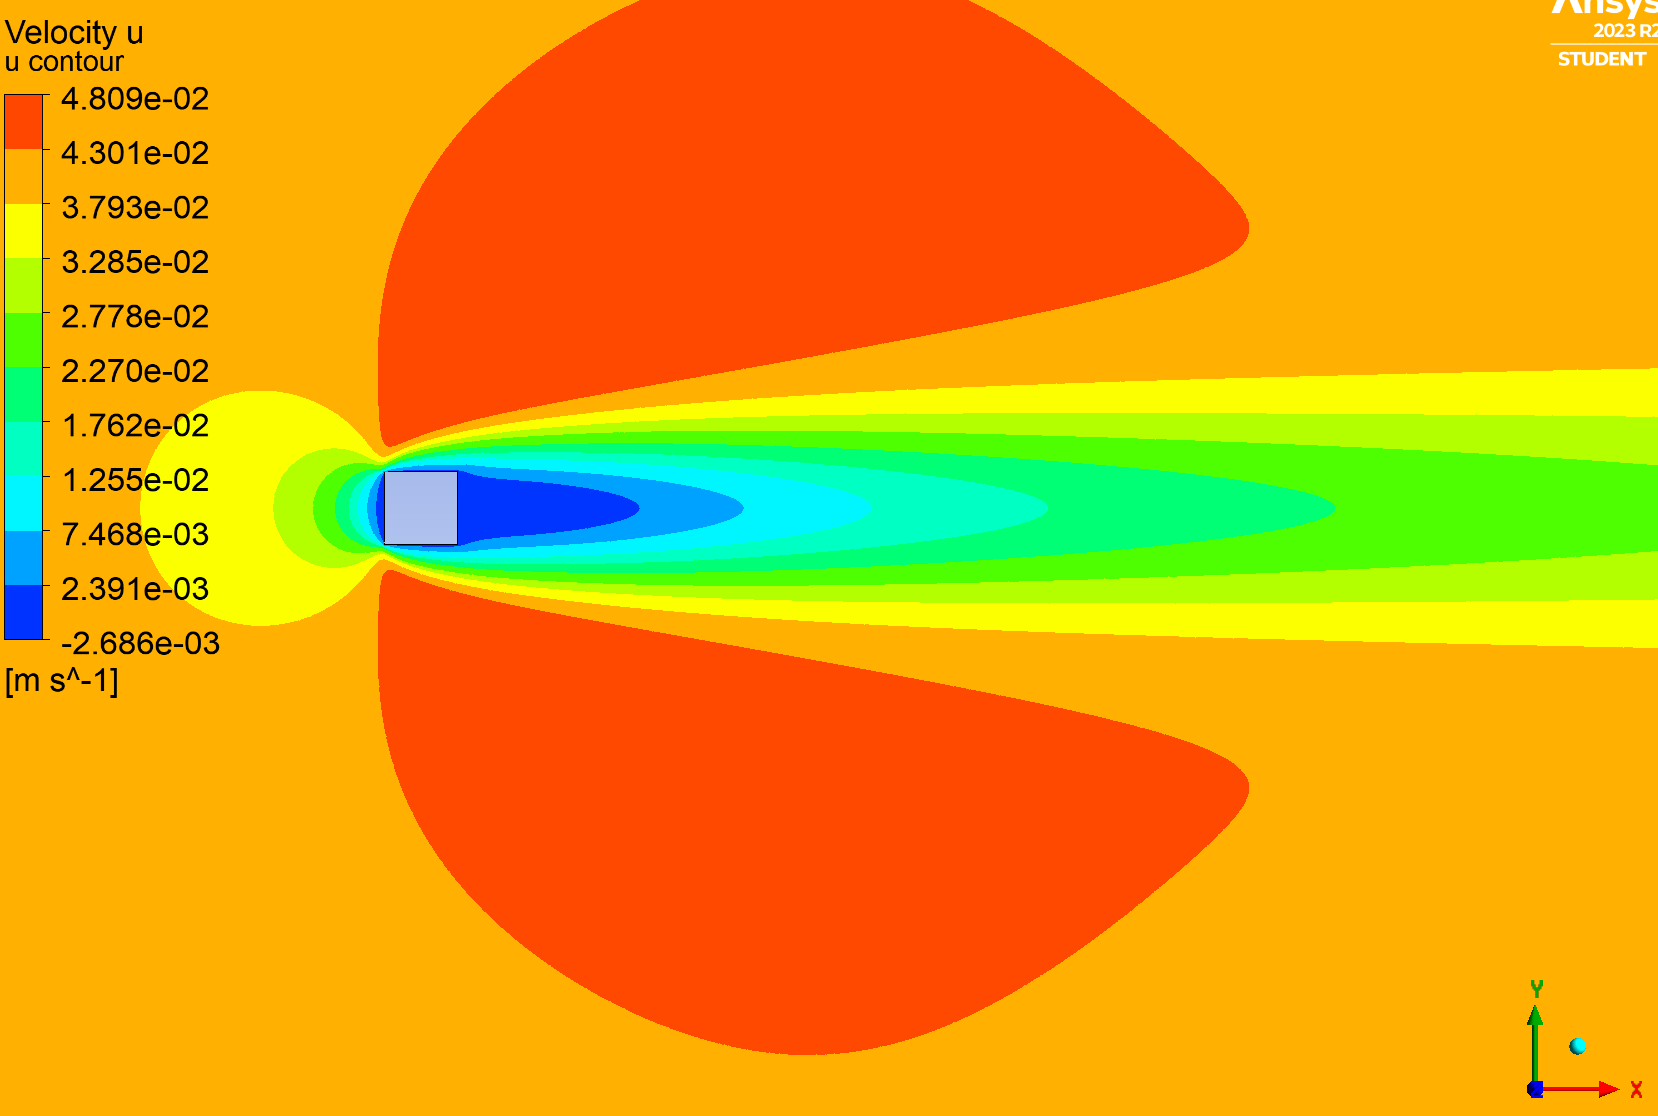
\includegraphics[width=\textwidth]{Questions/Figures/u velocity contour grid 5.png}
        \caption{Velocity Contour for Grid 5}
        \label{fig:velocity_contour_grid_5}
    \end{minipage}
\end{figure}
\begin{figure}[H]
    \centering
    \begin{minipage}{0.45\textwidth}
        \centering
        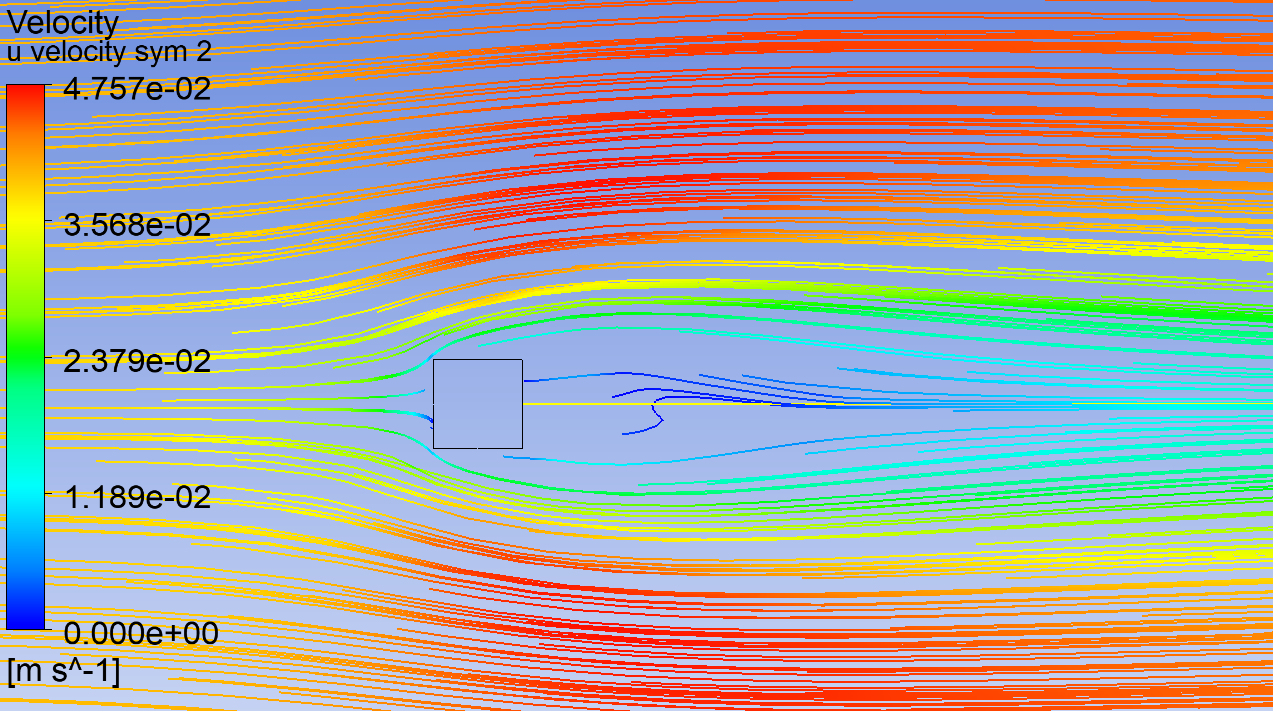
\includegraphics[width=\textwidth]{Questions/Figures/u velocity streamline grid 1.png}
        \caption{Streamlines for Grid 1}
        \label{fig:streamlines_grid_1}
    \end{minipage}
    \begin{minipage}{0.45\textwidth}
        \centering
        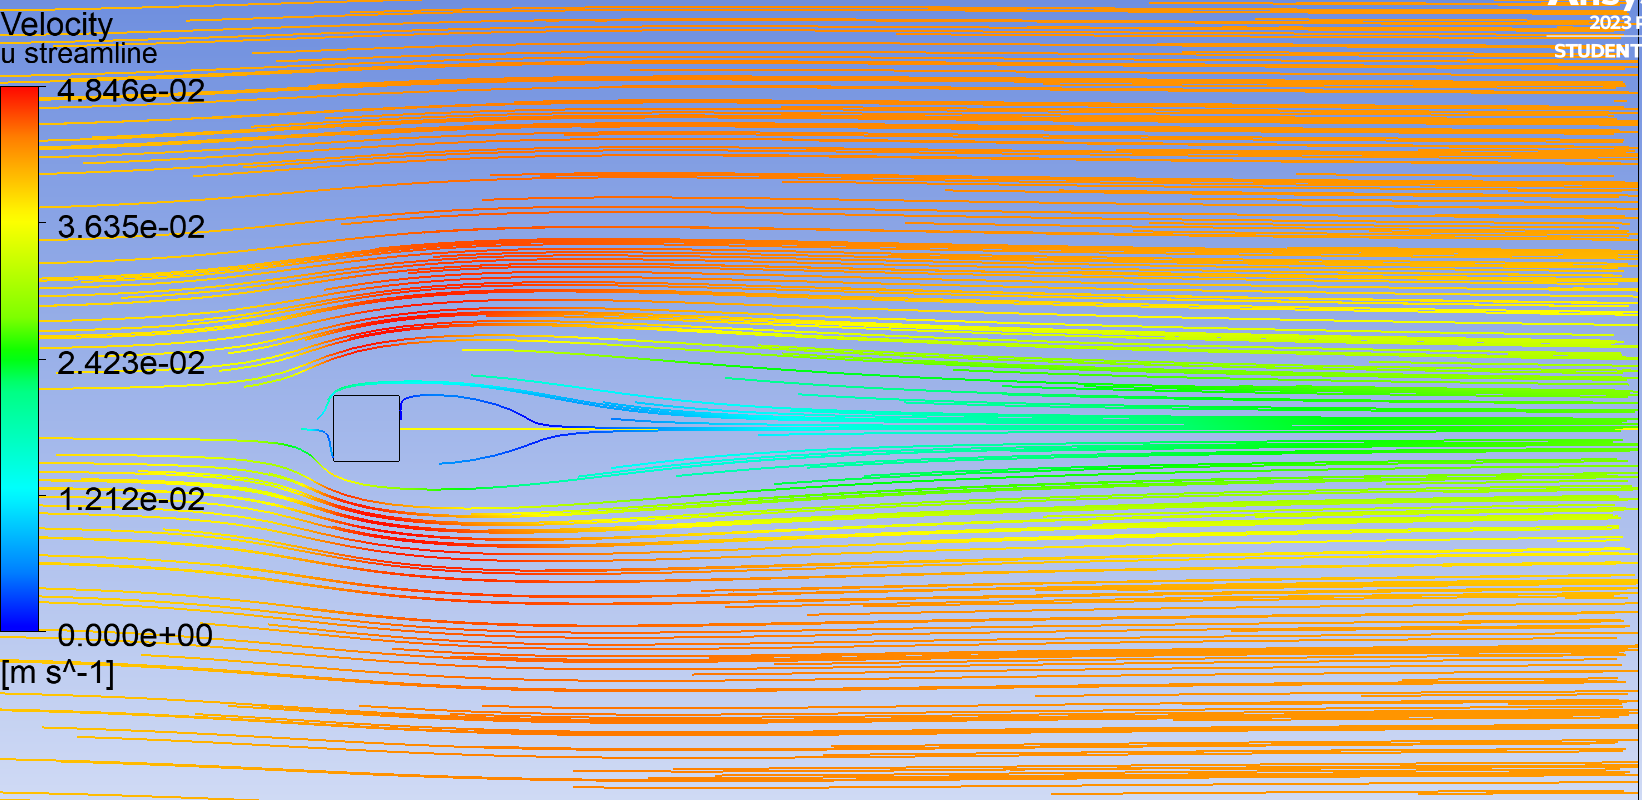
\includegraphics[width=\textwidth]{Questions/Figures/u velocity streamline grid 3.png}
        \caption{Streamlines for Grid 3}
        \label{fig:streamlines_grid_3}
    \end{minipage}
\end{figure}
\begin{figure}[H]
    \centering
    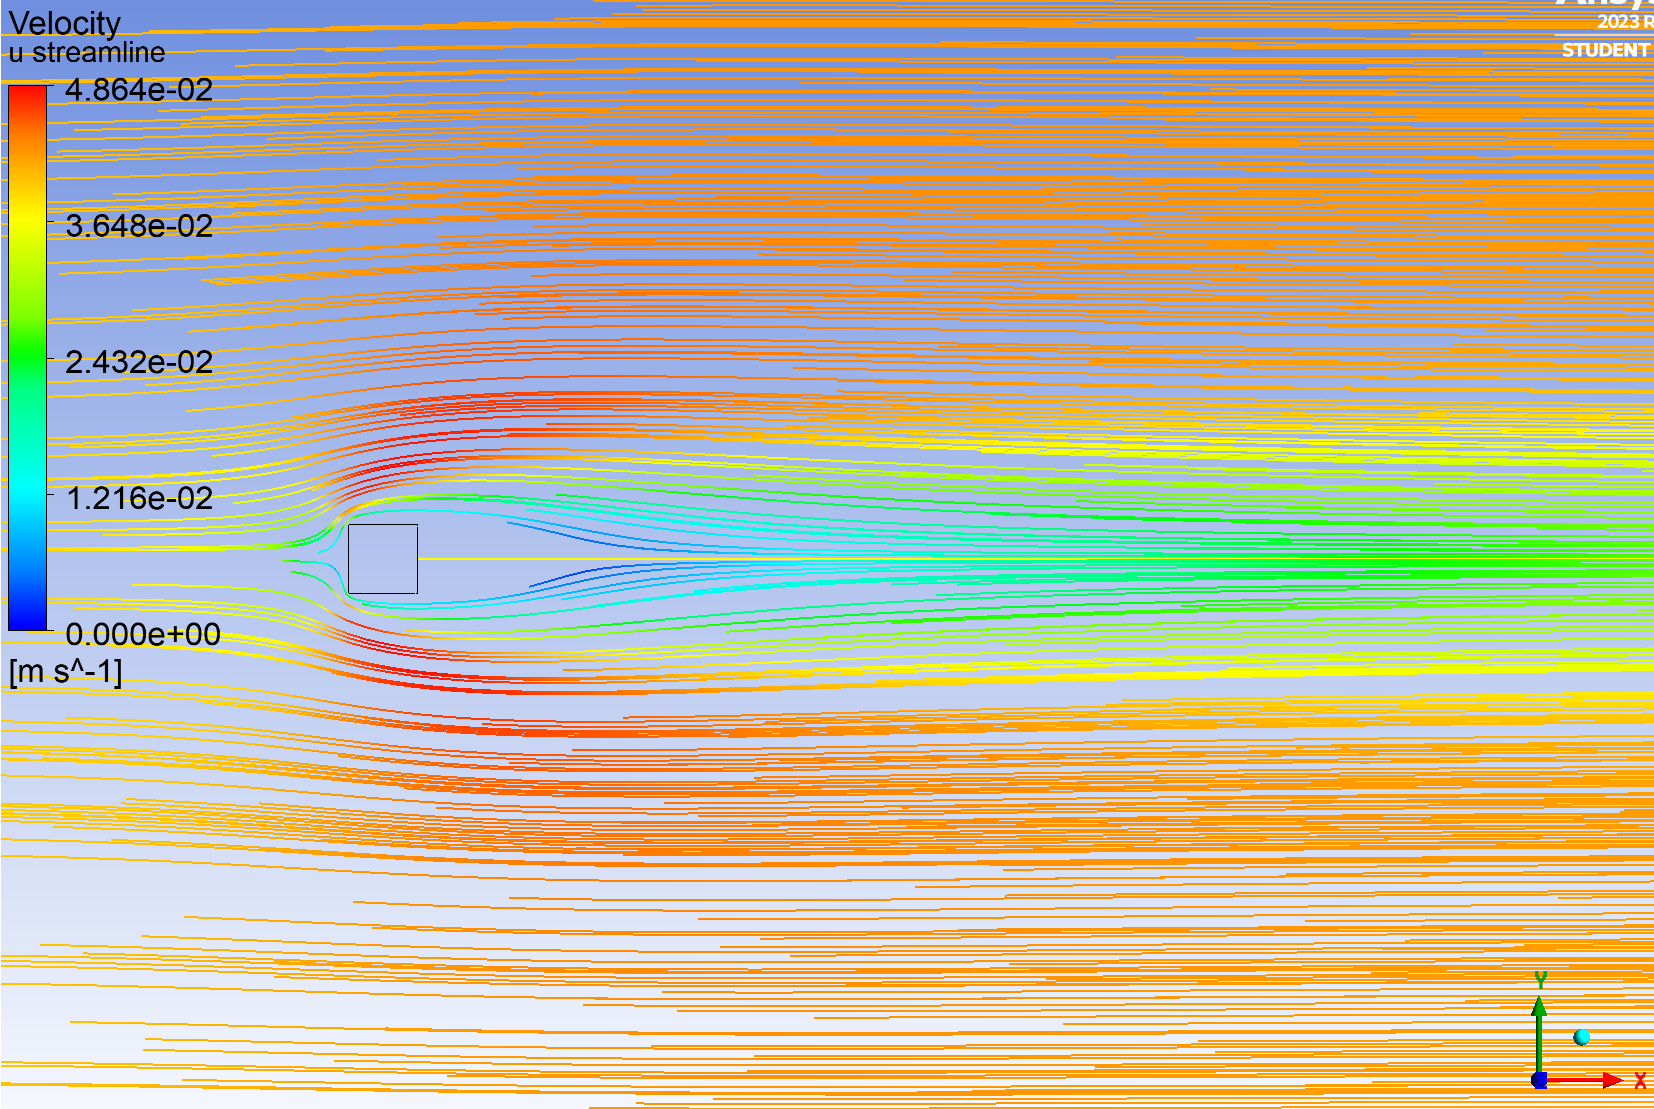
\includegraphics[width=0.45\textwidth]{Questions/Figures/u velocity streamline grid 5.png}
    \caption{Streamlines for Grid 5}
    \label{fig:streamlines_grid_5}
\end{figure}

\subsection{Drag Coefficient and Vortex Length}
\subsubsection{Vortex Length and Drag Coefficient}
The vortex length and drag coefficient are summarized in Table \ref{tab:vortex_length_drag_coefficient_summary}. 
\begin{table}[H]
    \centering
    \caption{Vortex Length and Drag Coefficient}
    \label{tab:vortex_length_drag_coefficient_summary}
    \begin{tabular}{cccc}
        \toprule
        Grid & Recirculation Length & Drag Coefficient \\
        & (m) & \\
        \midrule
        1 & 0.0115 & 3.1413 \\
        2 & 0.0181 & 2.7280 \\
        3 & 0.0186 & 2.5984 \\
        4 & 0.0183 & 2.5630 \\
        5 & 0.0183 & 2.5557 \\
        \bottomrule
    \end{tabular}
\end{table}
Sample calculations for grid 1 will be shown. The recirculation length is the distance between the two points ($x_1$, $x_2$) where the velocity is zero. Then
\begin{align*}
    L_r &= x_2 - x_1 \\
    &= 0.0234 - 0.0119 \\
    &= 0.0115 \text{ m}
\end{align*}
The drag coefficient is calculated as
\begin{align*}
    C_d &= \frac{2F_d}{\rho U_\infty^2 D} \\
    &= \frac{2 \times 2.51 \times 10^{-5}}{1.0 \times 0.04^2 \times 0.01} \\
    &= 3.1413
\end{align*}

\subsubsection{Recirculation Length on All Grids}
The combined plot of the velocity profile for all grids is shown in Figure \ref{fig:velocity_profile_all_grids}. Grid 1 does not really have a recirculation length, while grid 2 shows some recirculation. In Grids 3-5, asymptotic behavior is observed. The recirculation length seems to steady around grid 4, with grid 5 being almost indistinguishable. Grid 3 seems to capture the details of grids 4 and 5 for $\tilde{}$ 16x fewer cells.

\begin{figure}[H]
    \centering
    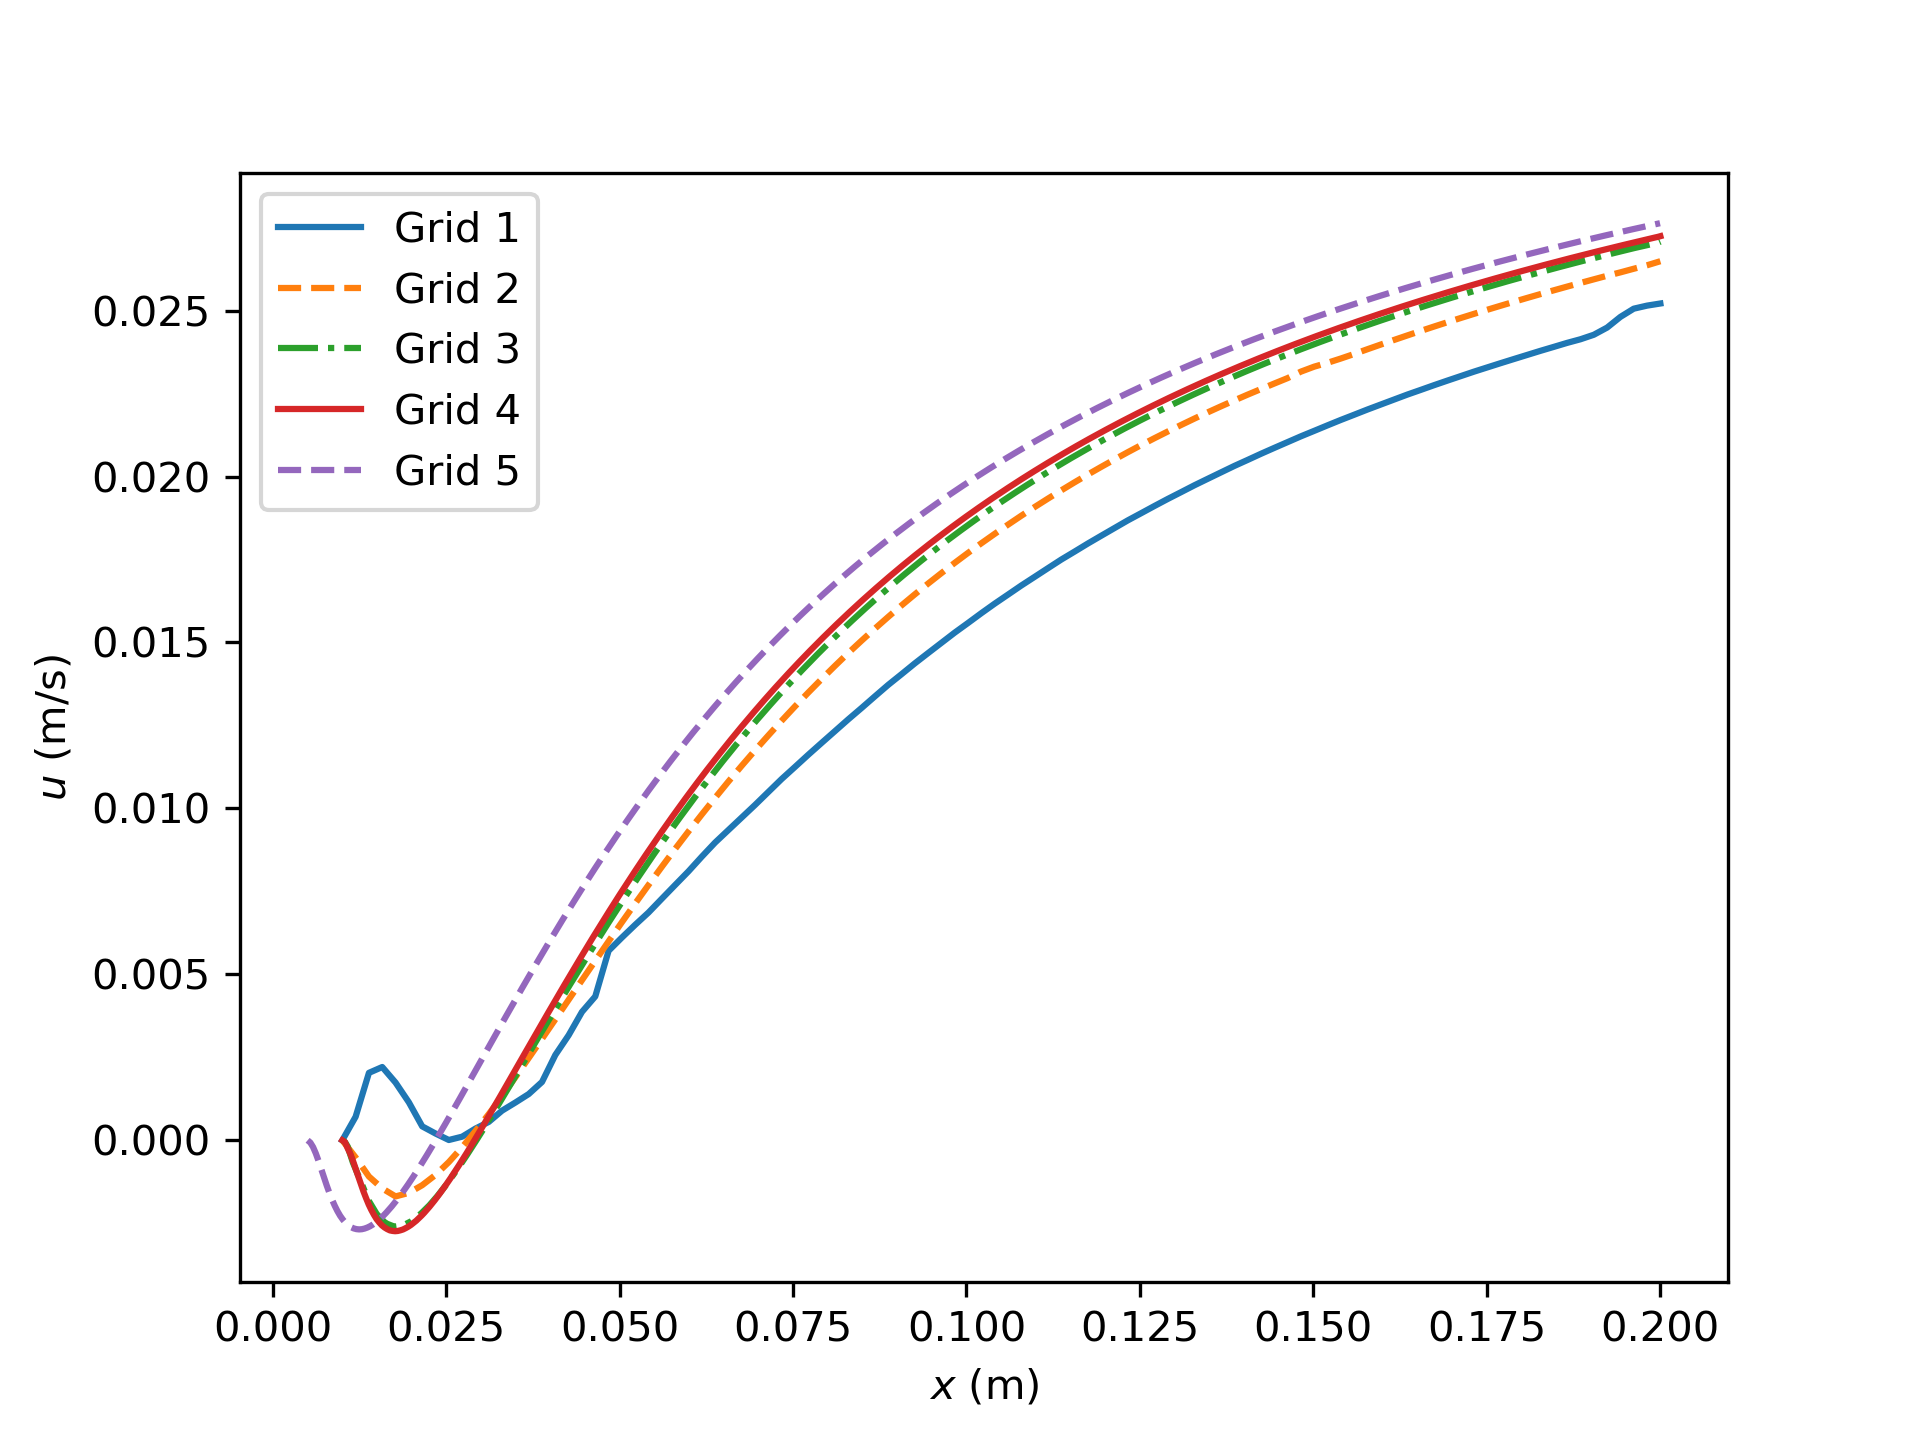
\includegraphics[width=0.5\textwidth]{Questions/Figures/recirc_combined.png}
    \caption{Velocity Profile for All Grids}
    \label{fig:velocity_profile_all_grids}
\end{figure}

\subsubsection{Mesh Independence}
\begin{figure}[H]
    \centering
    \begin{minipage}{0.45\textwidth}
        \centering
        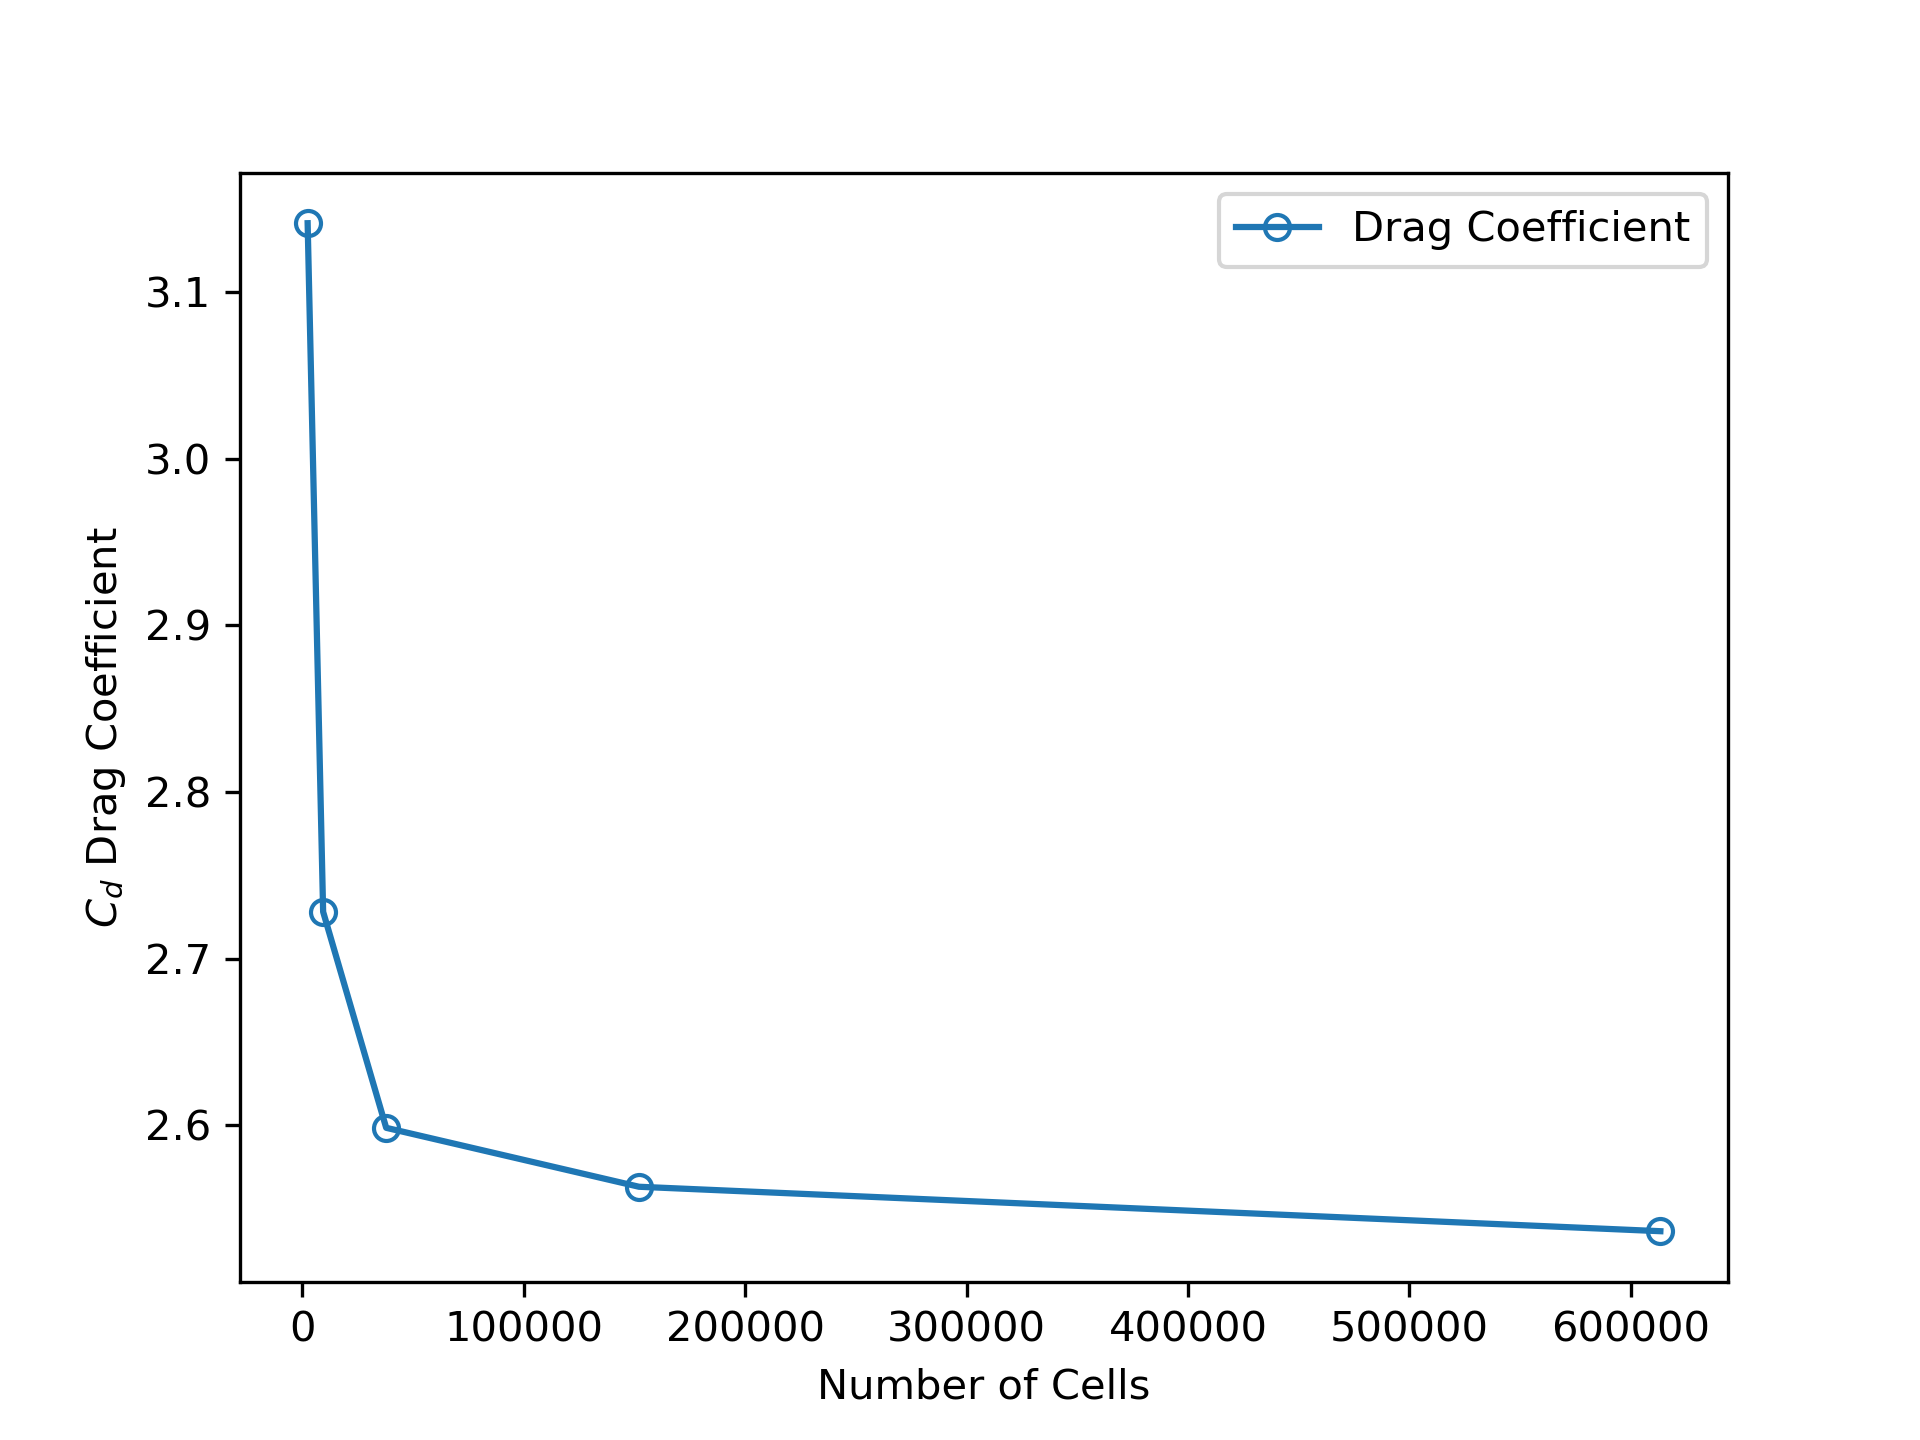
\includegraphics[width=\textwidth]{Questions/Figures/drag_coefficient_vs_cells.png}
        \caption{Drag Coefficient vs. Cells}
        \label{fig:drag_coefficient_vs_cells}
    \end{minipage}
    \begin{minipage}{0.45\textwidth}
        \centering
        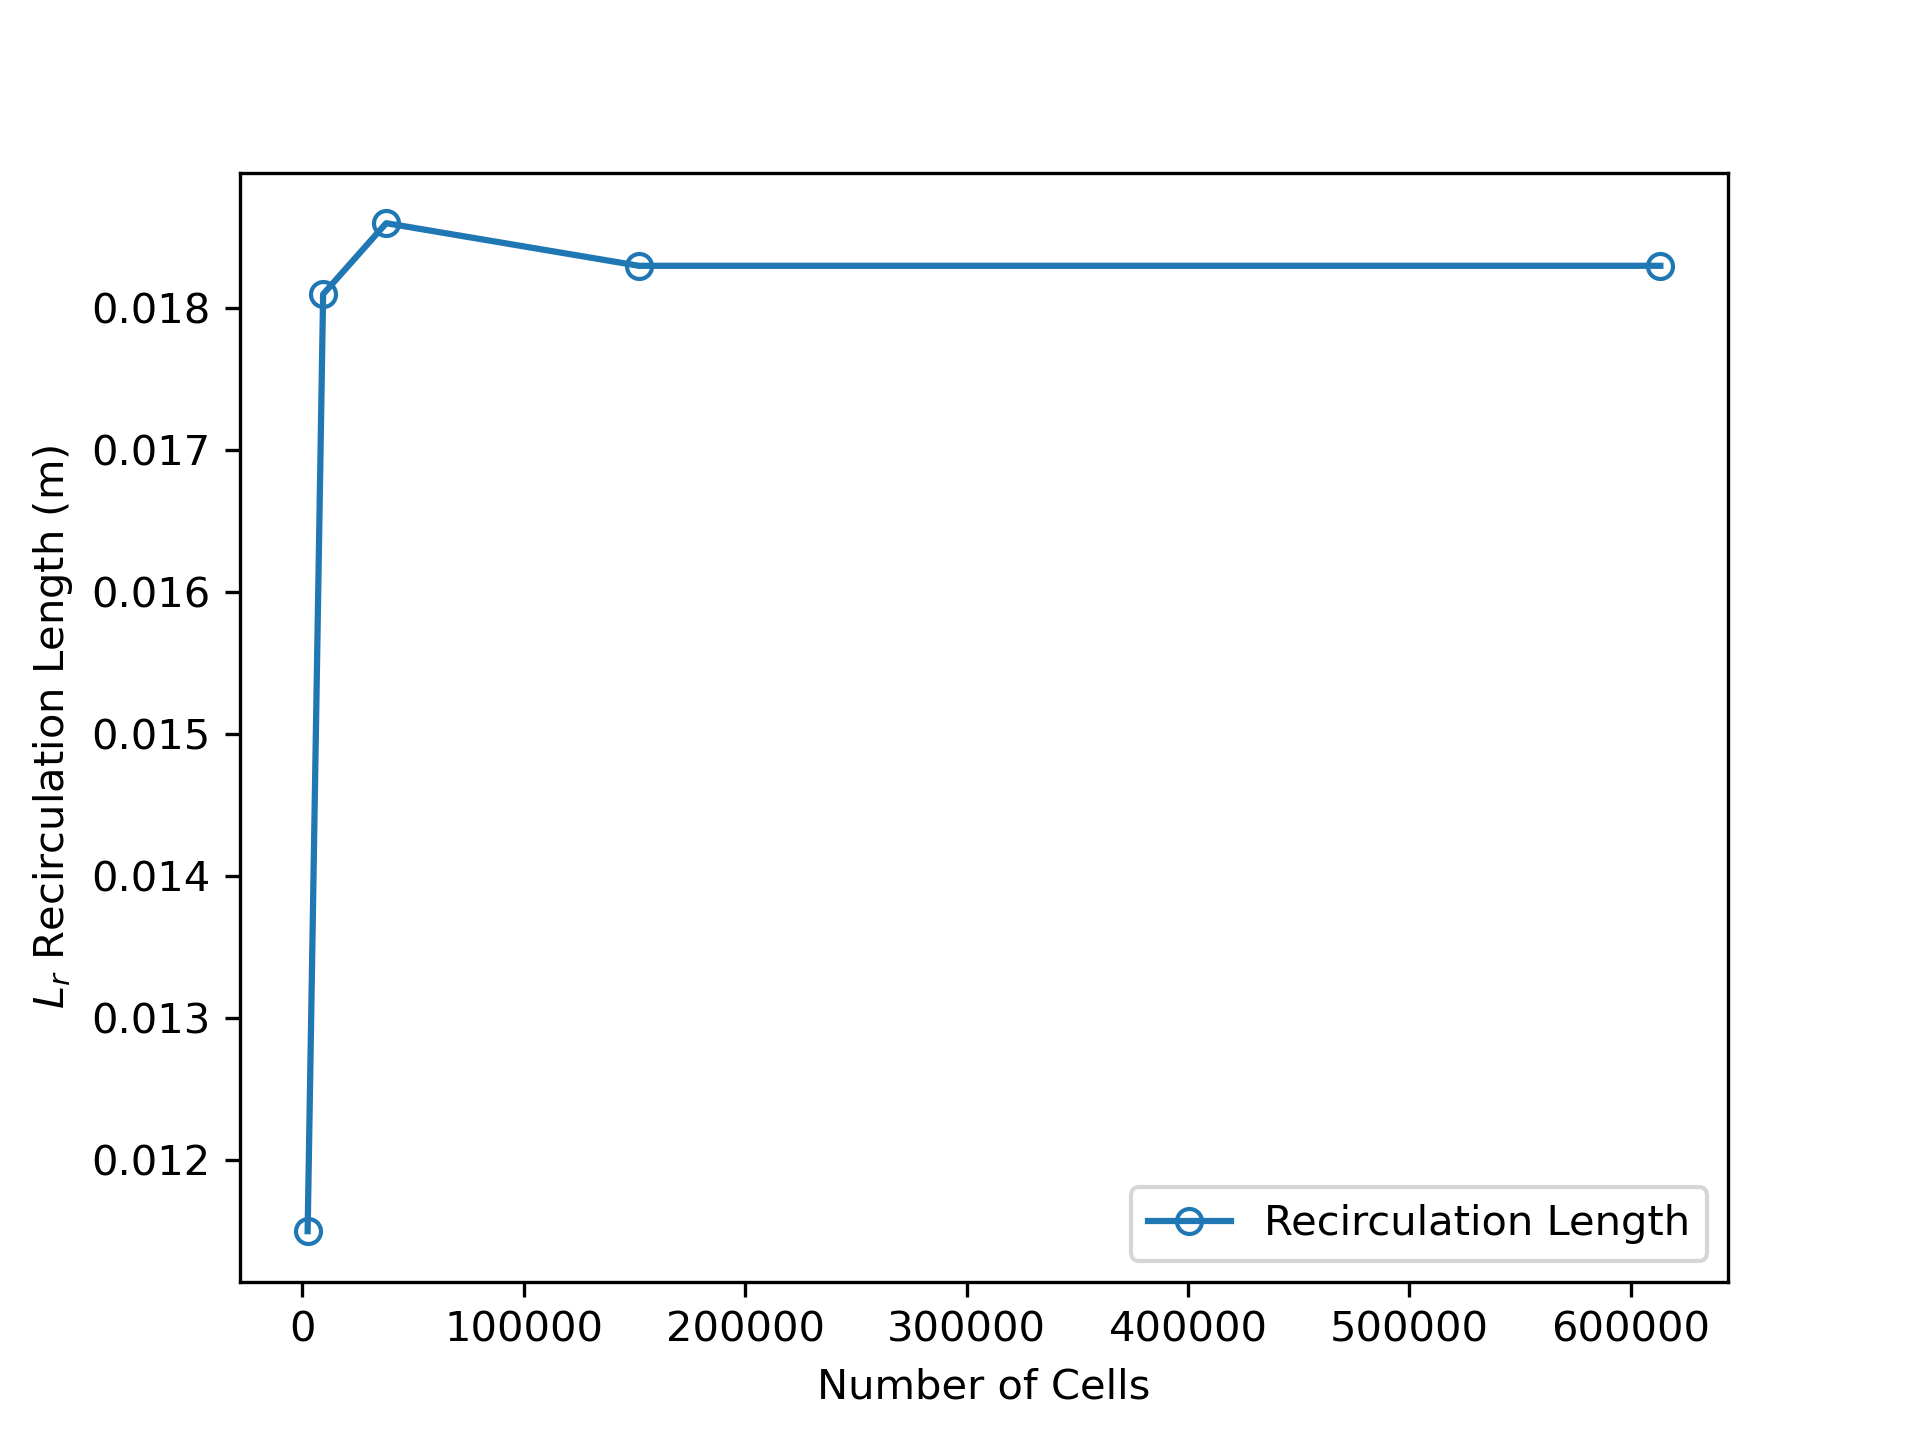
\includegraphics[width=\textwidth]{Questions/Figures/recirc_length_vs_cells.png}
        \caption{Recirculation Length vs. Cells}
        \label{fig:recirculation_length_vs_cells}
    \end{minipage}
\end{figure}
\begin{table}[H]
    \centering
    \caption{Error in Vortex Length and Drag Coefficient with Respect to Grid 5}
    \label{tab:error_vortex_length_drag_coefficient}
    \begin{tabular}{ccc}
        \toprule
        Grid & Vortex Length Error & Drag Coefficient Error \\
        & (\%) & (\%) \\
        \midrule
        1 & 37.16 & 22.92 \\
        2 & 1.09 & 6.75 \\
        3 & 1.64 & 1.67 \\
        4 & 0 & 0.29 \\
        5 & - & - \\
        \bottomrule
    \end{tabular}
\end{table}
The drag coefficient and recirculation length are plotted against the total number of cells in Figures \ref{fig:drag_coefficient_vs_cells} and \ref{fig:recirculation_length_vs_cells}. Asymptotic behavior is observed in both plots. Grid 3 is within 1.6\% of grid 5 for both the drag coefficient and recirculation length. The relative errors are summarized in Table \ref{tab:error_vortex_length_drag_coefficient}. 

\subsection{Estimation of the Order of the Method}
First calculate the order of the method. The order is calculated as
\begin{align*}
    p &\approx \frac{\log\left(\frac{F_{\Delta x_4} - F_{\Delta x_3}}{F_{\Delta x_5} - F_{\Delta x_4}}\right)}{\log a } \\
    &= \frac{\log\left(\frac{2.050 - 2.079}{2.045 - 2.050}\right)}{\log 2} \\
    &= \boxed{2.268}
\end{align*}
This is close to the expected value of 2. Therefore, the Richardson extrapolation can be used to estimate the exact drag coefficient. The error in the drag coefficient is calculated as
\begin{align*}
    \epsilon &= \frac{C_{\Delta x_5} - C_{\Delta x_4}}{a^p - 1} \\
    &= \frac{2.5557 - 2.5630}{2^{2.268} - 1} \\
    &= -0.001923
\end{align*}
then,
\begin{align*}
    C_{\text{exact}} &\approx C_{\Delta x_5} + \epsilon \\
    &= 2.5557 - 0.001923 \\
    &= \boxed{2.5537}
\end{align*}

\begin{figure}[H]
    \centering
    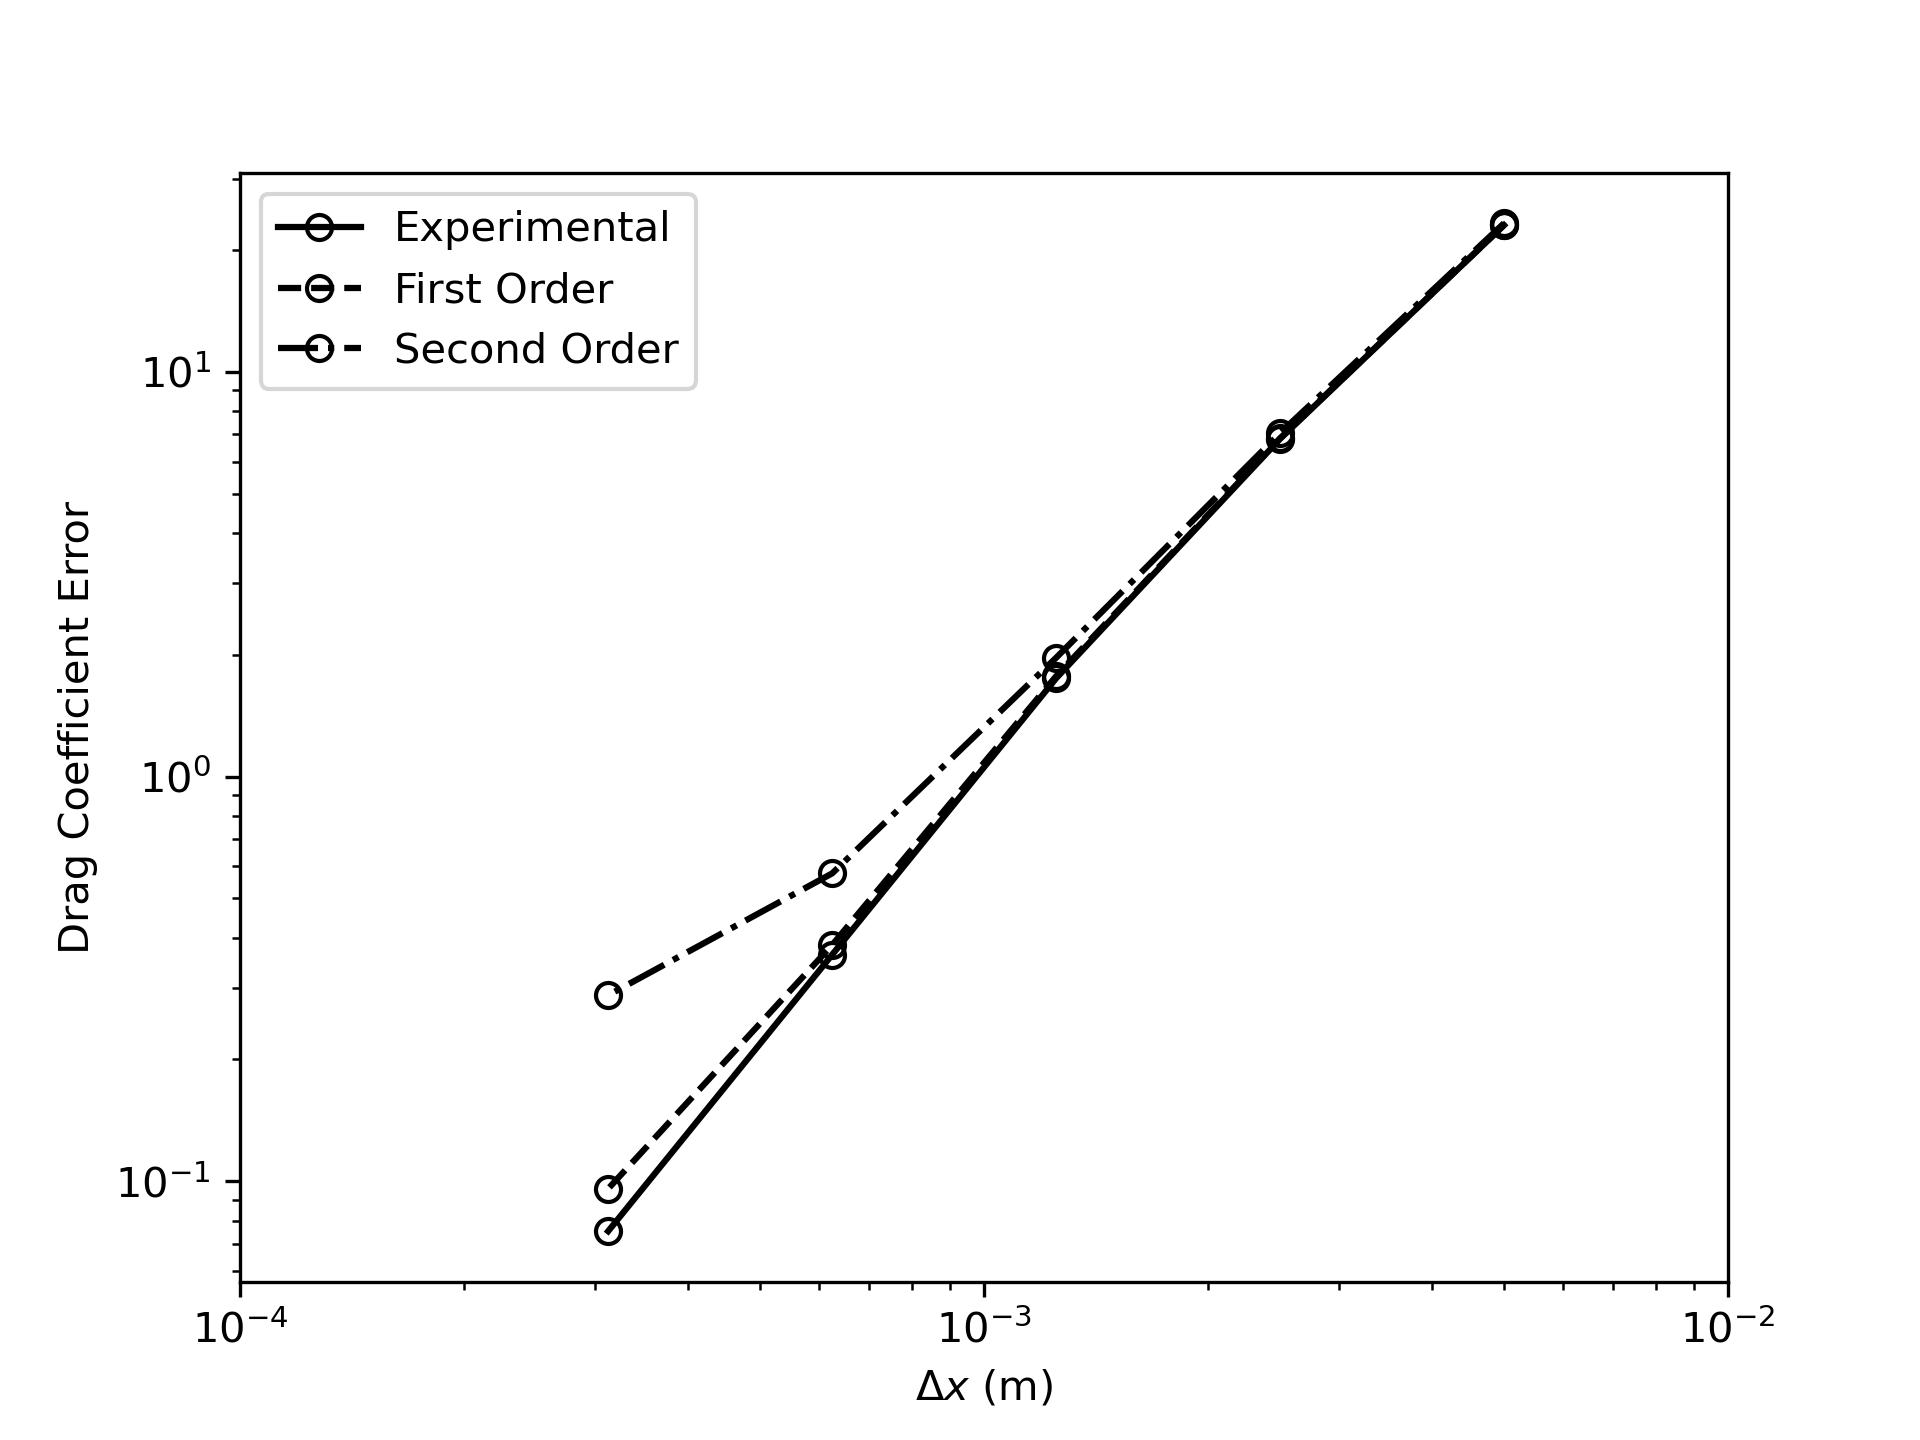
\includegraphics[width=0.5\textwidth]{Questions/Figures/richardson_error_vs_element_size.png}
    \caption{Error in Drag Coefficient vs. Element Size}
    \label{fig:richardson_error_vs_element_size}
\end{figure}
The error in the drag coefficient against the element size is shown in Figure \ref{fig:richardson_error_vs_element_size}. The experimental error decreases faster than the first and second order lines. This is consistent with the calculated order of the method being greater than 2. The data points from the experimental order and the second order are nearly coincident for the first 4 grids. 

The order of convergence being higher than 2 is likely due to some phenomena in the meshing process that is not accounted for in the theoretical order of the method. Further work could be performed to determine the exact cause of the higher order of convergence.

\subsection{Validation of the Results}
From another study, the drag coefficient was found to be 1.5657 at a Reynolds number of 60 \cite{paper}. The drag coefficient was found to be 2.5537 at a Reynolds number of 20, which is the same order of magnitude. The relative error is then
\begin{align*}
    \text{Relative Error} &= \frac{2.5537 - 1.5657}{1.5657} \\
    &= \boxed{63.1\%}
\end{align*}
This is a large error, but the Reynolds number is three times smaller than the Reynolds number in the other study. 

Since Reynolds number is low, this can be approximated as Stokes flow. Since density vanishes in Stokes flow, it can be shown from Buckingham Pi theorem that drag is a function of speed, length, and viscosity. Written mathematically, 
\begin{align*}
    F_d &= C_1\mu U_\infty D
\end{align*}
where $C_1$ is a constant dependent on the geometry. The drag coefficient is then
\begin{align*}
    C_d &= \frac{2F_d}{\rho U_\infty^2 D} \\
    &= \frac{2 C_1 \mu U_\infty D}{\rho U_\infty^2 D} \\
    &= \boxed{\frac{C_2}{\text{Re}}}
\end{align*}
Thus, the drag coefficient is inversely proportional to the Reynolds number in Stokes flow. It is reasonable that the drag coefficient would be larger at a lower Reynolds number. The results are within the same order of magnitude, so the results are reasonable.
\\\\
\noindent \textbf{Note:} I reran the simulation on grid 5 with Re = 60 and found the drag coefficient to be 1.6962, which is within 8.3\% of the other study. This suggests that the error in the original simulation is due to the Reynolds number difference.